%%%%%%%%%%%%%%%%%%%%%%%%%%%%%%%%%%%%%%%%%%%%%%%%%%%%%%%%%
 % Zawartość tego projektu jest niemodyfikowalna. 
 % Jeżeli chcesz wprowadzić w nim zmiany, to musisz utworzyć jego kopię — patrz https://www.overleaf.com/learn/how-to/Copying_a_project
 %%%%%%%%%%%%%%%%%%%%%%%%%%%%%%%%%%%%%%%%%%%%%%%%%%%%%%%%%
 %
 %	Name			:: 	The official template for the typesetting of diploma theses at the Faculty of Computer Science of AGH University of Krakow
 %	Author			:: 	Stanisław Polak (polak[aT]icsr[DoT]agh[DoT]edu[DoT]pl)
 %	Created			::	2024-02-14
 %	Modified	    ::	2024-03-04
 %	Version			:: 	1.3.1
 %	Email			:: 	polak[aT]icsr[DoT]agh[DoT]edu[DoT]pl
 %	Website			:: 	http://www.icsr.agh.edu.pl/~polak/
 %   Youtube         ::  https://www.youtube.com/user/spolak69
 %   Github          ::  https://github.com/polaksta
 %	License			:: 	This work may be distributed and/or modified under the
 %                       conditions of the LaTeX Project Public License, either version 1.3
 %                       of this license or (at your option) any later version.
 %                       The latest version of this license is in
 %                       http://www.latex-project.org/lppl.txt
 %                       and version 1.3 or later is part of all distributions of LaTeX
 %                       version 2005/12/01 or later.
 %
 %	Description		::	This document is a demonstration of the template
 %
 %%%%%%%%%%%%%%%%%%%%%%%%%%%%%%%%%%%%%%%%%%%%%%%%%%%%%%%%%
 % Niniejszy dokument — szkielet pracy dyplomowej — prezentuje przykłady użycia klasy 'agh-wi' oraz pakietów tradycyjnie używanych w pracach
 % dyplomowych z informatyki. Dla kilku z nich, wartości początkowe parametrów konfiguracyjnych są zdefiniowane 
 % w klasie  — wartości te uwzględniają uwagi osób prowadzących przedmiot "Pracownia Dyplomowa". 
 % Oczywiście możesz używać dowolnych pakietów, niekoniecznie tych, które są pokazane w tym dokumencie
 %%%%%%%%%%%%%%%%%%%%%%%%%%%%%%%%%%%%%%%%%%%%%%%%%%%%%%%%%
 % Poniższe uwagi NIE DOTYCZĄ Overleaf-a
 %%%%%%%%%%%%%%%%%%%%%%%%%%%%%%%%%%%%%%%%%%%%%%%%%%%%%%%%%
 % W tej przykładowej pracy dyplomowej użyto, między innymi, pakietów:
 %   - "minted", co oznacza, że musisz uruchomić kompilator z opcją '-shell-escape'
 %   - "biblatex", co oznacza, że po kompilacji (dokumentu) musisz, jeszcze, wygenerować plik '.bbl'
 %   - "nomencl", co oznacza, że za pomocą komendy 'makeindex' musisz wygenerować wykaz symboli
 %
 % Tak więc, w celu wygenerowania wynikowego dokumentu PDF, musisz wykonać następujące komendy:
 %       pdflatex -shell-escape example
 %       biber example
 %       makeindex example.nlo  -s nomencl.ist -o example.nls
 %       pdflatex -shell-escape example
 %       pdflatex -shell-escape example
 %
 % Dodatkowo musisz mieć zainstalowany program 'pygmentize', który jest częścią pakietu "Pygments" (https://pygments.org/)
 % Ww. programy powinny zainstalować się automatycznie podczas instalacji pakietów LaTeX
 %
 % Jeżeli masz zainstalowany program 'latexmk', to możesz wygenerować dokument PDF następująco:
 %       latexmk example
 %       makeindex example.nlo  -s nomencl.ist -o example.nls
 %       latexmk example
 %
 % Do edycji (oraz komplilacji) dokumentów LaTeX polecam program 'TeXstudio' (https://www.texstudio.org/)
 %
 % Autor: Stanisław Polak <polak[aT]agh[DoT]edu[DoT]pl>
 %%%%%%%%%%%%%%%%%%%%%%%%%%%%%%%%%%%%%%%%%%%%%%%%%%%%%%%%%
 \documentclass[data-science]{agh-wi} % Praca po polsku; na stronie tytułowej, najpierw jest widoczny polskojęzyczny tytuł, a potem angielskojęzyczny.
 % Kierunek 'Informatyka'.
 % Przeznaczona do oglądania przy użyciu przeglądarki PDF.
%%%%%%%%%%%%%%%%%%%%%%%%%%%%%%%%%
% Inne, przykładowe, użycia klasy
%%%%%%%%%%%%%%%%%%%%%%%%%%%%%%%%%
% \documentclass[english]{agh-wi}               % Praca po angielsku; 
                           %     strona tytułowa po polsku, ale najpierw jest widoczny angielskojęzyczny tytuł, a potem polskojęzyczny.  
                           % Kierunek 'Informatyka'.
                           % Przeznaczona do oglądania przy użyciu przeglądarki PDF.
% \documentclass[english, data-science]{agh-wi} % Praca po angielsku; ...
                           % Kierunek 'Informatyka - Data Science'.
                           % Przeznaczona do oglądania przy użyciu przeglądarki PDF.
% \documentclass[print]{agh-wi}                 % Praca po polsku; ...
                           % Kierunek 'Informatyka'.
                           % Przeznaczona do drukowania - każda strona posiada,
                           %    dodatkowy (2cm), margines na oprawę.
%%%%%%%%%%%%%%%%%%%%%%%%%%%%%%%%%%%%%
% Parametry dla strony tytułowej
%%%%%%%%%%%%%%%%%%%%%%%%%%%%%%%%%%%%%
\titlePL{Generowanie muzyki przy pomocy dużych modeli językowych}  % Tytuł po polsku
\titleEN{Music generation with Lange Language Models} % Tytuł po angielsku
\author{Filip Ręka}
\supervisor{dr hab. Maciej Smołka prof. AGH}
%%%%%%%%%%%%%%%%%%%%%%%%%%%%%%%%%%%%%
% Pakiety
%%%%%%%%%%%%%%%%%%%%%%%%%%%%%%%%%%%%%
% Podstawowe — na pewno będziesz ich potrzebował(a) w swojej wersji pracy dyplomowej
%%%%%%%%%%%%%%%%%%%%%%%%%%%%%%%%%%%%%
\usepackage{polski} % Obsługa języka polskiego
%%%%%%%%%%%%%%%%%%%%%%%%%%%%%%%%%%%%%
% Dodatkowe — niekoniecznie będziesz ich potrzebował(a) w swojej wersji pracy dyplomowej
%%%%%%%%%%%%%%%%%%%%%%%%%%%%%%%%%%%%%
\usepackage[sorting=none]{biblatex}           % Spis literatury ma być tworzony na podstawie zawartości bibliograficznej bazy danych
\usepackage{amsmath}                          % Dodatkowe środowiska matematyczne
\usepackage{amssymb}                          % Dodatkowe symbole matematyczne
\usepackage[polish, intoc]{nomencl}           % Definiowanie symboli
\usepackage{graphicx}                         % Wstawianie grafik zewnętrznych
\usepackage{xcolor}                           % Kolorowy tekst
\usepackage{tabularx}                         % Rozszerzona wersja środowiska 'tabular'
\usepackage{longtable}                        % Skład "długich" tabel
\usepackage[ruled,linesnumbered]{algorithm2e} % Algorytmy w formie pseudokodu
\usepackage{listings}                         % Formatowanie kodów źródłowych programów
\usepackage[newfloat]{minted}                 % Formatowanie kodów źródłowych programów
\usepackage{hyperref}                         % Obsługa adresów URL — zbędny jeżeli używasz 'biblatex'
\usepackage{csquotes}                         % Polskie cudzysłowy — rekomendowany jeżeli używasz 'biblatex'
\usepackage{tocloft}
\usepackage{float}
\usepackage{musicography}
\usepackage{array}
\usepackage{pgfplots}
\usepackage{pgfplotstable}
\usepackage{filecontents}
% \usepackage[draft,nosingleletter]{impnattypo}
\begin{filecontents}{data.dat}
    date  Mamba_60M  Mamba_6M  GPT2_60M  GPT2_6M
    128   1.910      1.360     2.418     1.125
    256   1.613      1.159     2.515     0.628
    512   1.610      2.407     3.574     0.903
    1024  1.638      4.518     3.565     0.885
    2048  1.618      5.133     3.562     0.901
    4096  1.614      5.144     3.717     0.904
    8192  1.660      5.146     3.571     0.904
    16384 1.776      5.234     3.556     0.906
\end{filecontents}

% NAJWAŻNIEJSZE POLECENIE
\newcommand{\shrug}[1][]{%
\begin{tikzpicture}[baseline,x=0.8\ht\strutbox,y=0.8\ht\strutbox,line width=0.125ex,#1]
\def\arm{(-2.5,0.95) to (-2,0.95) (-1.9,1) to (-1.5,0) (-1.35,0) to (-0.8,0)};
\draw \arm;
\draw[xscale=-1] \arm;
\def\headpart{(0.6,0) arc[start angle=-40, end angle=40,x radius=0.6,y radius=0.8]};
\draw \headpart;
\draw[xscale=-1] \headpart;
\def\eye{(-0.075,0.15) .. controls (0.02,0) .. (0.075,-0.15)};
\draw[shift={(-0.3,0.8)}] \eye;
\draw[shift={(0,0.85)}] \eye;
% draw mouth
\draw (-0.1,0.2) to [out=15,in=-100] (0.4,0.95); 
\end{tikzpicture}}

%%%%%%%%%%%%%%%%%%%%%%%%%%%%%%%%%%%%
%  % Konfiguracja rysunków TikZ
%%%%%%%%%%%%%%%%%%%%%%%%%%%%%%%%%%%%
\usetikzlibrary{shapes.geometric,arrows.meta,arrows,matrix,fit, positioning} 
\tikzstyle{every picture}+=[remember picture]
\tikzstyle{na} = [baseline=-.5ex]
%%%%%%%%%%%%%%%%%%%%%%%%%%%%%%%%%%%%
% Ładowanie danych bibliograficznych
%%%%%%%%%%%%%%%%%%%%%%%%%%%%%%%%%%%%
\addbibresource{bibliography.bib}
%%%%%%%%%%%%%%%%%%%%%%%%%%%%%%%%%%%%%
% Opcje konfiguracyjne pakietów
%%%%%%%%%%%%%%%%%%%%%%%%%%%%%%%%%%%%%
% Pakiet 'framed'
\definecolor{shadecolor}{gray}{0.9}
% Pakiet 'nomencl'
\makenomenclature % Otwórz plik 'example.nlo'
%%%%%%%%%%%%%%%%%%%%%%%%%%%%%%%%%%%%%
% Definicje komend
%%%%%%%%%%%%%%%%%%%%%%%%%%%%%%%%%%%%%
\newcommand{\alert}[1]{\colorbox{red!50}{#1}}
%%%%%%%%%%%%%%%%%%%%%%%%%%%%%%%%%%%%%
% Twierdzenia i podobne struktury
%%%%%%%%%%%%%%%%%%%%%%%%%%%%%%%%%%%%%
\newtheorem{theorem}{Twierdzenie}
\newtheorem{definition}{Definicja}

%%%%%%%%%%%%%%%%%%%%%%%%%%%%%%%%%%%%%
% Ustawienie licznika do subsubsection
%%%%%%%%%%%%%%%%%%%%%%%%%%%%%%%%%%%%%
\setcounter{secnumdepth}{5}

\newcounter{comment}[chapter]
\newenvironment{comment}[1][]{\begin{shaded}\refstepcounter{comment}
\noindent \textbf{Uwaga~\thechapter.\thecomment. #1} \rmfamily}{\end{shaded}}
%%%%%%%%%%%%%%%%%%%%%%%%%%%%%%%%%%%%%
%%%%%%%%%%%%%%%%%%%%%%%%%%%%%%%%%%%%%
\begin{document}
%%%%%%%%%%%%%%%%%%%%%%%%%%%%%%%%%%%%%
\frontmatter % Część wstępna
%%%%%%%%%%%%%%%%%%%%%%%%%%%%%%%%%%%%%
\maketitle % Dodaj stronę tytułową
%%%%%%%%%%%%%%%%%%%%%%%
% Jeżeli chcesz komuś podziękować, to możesz użyć poniższego kodu

%%%%%%%%%%%%%%%%%%%%%%%
\begin{abstractPL}
    Praca poświęcona jest eksploracji możliwości generowania muzyki przy pomocy dużych modeli językowych (\textit{Large Language Models} LLM). Celem badania jest analiza architektur modeli językowych i ich zastosowanie w procesie tworzenia muzyki. Praca skupia się na podobieństwach strukturalnych między muzyką a tekstem, argumentując, że te dwie formy ekspresji dzielą wspólne cechy sekwencyjne, co pozwala na adaptację modeli językowych do generowania muzycznych kompozycji. W pracy przedstawiono również przegląd istniejących formatów cyfrowej reprezentacji muzyki oraz zbiory danych, które mogą być użyte do treningu modeli generatywnych. Przez przeprowadzenie serii eksperymentów, w których wykorzystano różnorodne architektury, takie jak transformery i modele przestrzeni stanów, przeanalizowano efektywność różnych podejść w kontekście generowania muzyki. Została podjęta próba oceny wygenerowanych fragmentów muzycznych przy pomocy dostępnych modeli LLM, które są udostępniane komercyjnie lub zostały wytrenowane, aby rozumieć muzykę. Praca oferuje nowe perspektywy na temat potencjału LLM w dziedzinie sztucznej kreatywności muzycznej, otwierając drogę do dalszych badań w tej fascynującej przestrzeni interdyscyplinarnej.
\end{abstractPL}
\begin{abstractEN}
    The work is devoted to exploring the possibilities of music generation using large language models (LLMs). The aim of the study is to analyze the architectures of language models and their application in the process of music creation. The paper focuses on the structural similarities between music and text, arguing that these two forms of expression share common sequential features, which allows the adaptation of language models for the generation of musical compositions. The paper also provides an overview of existing formats for digital representation of music and datasets that can be used to train generative models. By conducting a series of experiments using a variety of architectures, such as transformers and state space models, the effectiveness of different approaches in the context of music generation was analyzed. An attempt was made to evaluate the generated musical fragments using commercially available LLM models or those trained to understand music. The work offers new perspectives on the potential of LLM in the field of artificial musical creativity, paving the way for further research in this fascinating interdisciplinary space.
\end{abstractEN}
%%%%%%%%%%%%%%%%%%%%%%%%%%%%%%%%%%%%%
%%%%%%%%%%%%%%%%%%%%%%%%%%%%%%%%%%%%%
% \setlength{\cftsecnumwidth}{4em} % Adjust according to your needs
% \setlength{\cftsubsubsecindent}{8em} % Adjust according to your needs
% \setcounter{tocdepth}{5}
\tableofcontents   % Wygeneruj spis treści
\newpage
\listoffigures     % Wygeneruj listę rysunków
\listoftables      % Wygeneruj listę tabel
% \listofalgorithms  % Wygeneruj listę algorytmów
% Wygeneruj listę kodów źródłowych
% \lstlistoflistings % Jeżeli do tworzenia listingów używasz pakietu 'listings'
% \listoflistings % Jeżeli do tworzenia listingów używasz pakietu 'minted'
% \printnomenclature % Wyświetl listę symboli
%%%%%%%%%%%%%%%%%%%%%%%%%%%%%%%%%%%%%
\mainmatter % Część główna
%%%%%%%%%%%%%%%%%%%%%%%%%%%%%%%%%%%%%
\chapter{Wstęp}
Muzyka od zawsze stanowiła istotny element ludzkiego życia, inspirując, emocjonując \\i łącząc ludzi na różnych poziomach. Tradycyjnie proces tworzenia muzyki był zarezerwowany dla utalentowanych muzyków i kompozytorów, którzy posiadali wyjątkowy dar jej tworzenia. Jednakże, w erze cyfrowej, której towarzyszy rozwój sztucznej inteligencji, pojawiają się nowe możliwości w dziedzinie generowania muzyki. Modelowanie generatywne, będące obszarem sztucznej inteligencji, pozwala na tworzenie nowych danych, w tym również muzyki, na podstawie wzorców i reguł wykrytych w zbiorze treningowym. Dynamiczny rozwój dziedziny przetwarzania języka naturalnego (NLP) ukazuje skuteczność tego podejścia w problemach generowania danych sekwencyjnych, do których należy właśnie tekst oraz muzyka.
\section{Motywacja}
Przez ostatnie lata widzimy szybki rozwój dużych modeli językowych (LLM), które\\ w szczególnie dobry sposób radzą sobie z rozumieniem tekstu w wielu językach. Modele\\ te uczone są na wielkich korpusach danych, przez co są w stanie nauczyć się słownictwa oraz zasad gramatyki, a nastepnie na podstawie zapytania udzielonego przez użytkownika wygenerować odpowiednią odpowiedź. Modele te znalazły zastosowanie w maszynowej translacji tekstu, analizie sentymentu, odpowiadaniu na pytania użytkownika czy generowania kodu na podstawie poleceń oraz kontekstu nawet dużych projektów. Muzyka swoją strukturą jest bardzo podobna do tekstu. Każda nuta, tak jak słowo jest zależna nie tylko od tych, które występują przed nią, ale również od szerszego kontekstu utworu jak również i tonacji w której dany utwór został napisany. Wykonując to porównanie, można łatwo zauważyć, dlaczego modele analizujące tekst oraz język pisany są potencjalnie dobrymi kandydatami do próby analizy i generowania muzyki. Obecnie w celach generatywnych stosuje się modele o bardzo dużej ilości parametrów, przez co nie są one często dostępne dla przeciętnego użytkownika który nie posiada dedykowanego sprzętu. Dodatkowym utrudnieniem jest typowa architektura oparta o transformer, który jest bardzo dobrym wyborem w tego rodzaju zadaniach, jednak generowanie danych przy jego pomocy jest wolne. Obecnie pojawiają się nowe modele do zadań NLP, które jeszcze nie zostały dobrze zbadane w zadaniach muzycznych, a rozwiązują problemy modeli transformerowych. Podejście do generowania muzyki w sposób podobny do metod używanych w generacji tekstu może skutkować powstaniem analogicznych narzędzi, czyli na przykład programów do autouzupałniania melodii. Artyści korzystający z narzędzi do tworzenia muzyki mogliby otrzymywać podpowiedzi od modelu, który na podstawie już stworzonej przez artystę muzyki, generowałby możliwe jej zakończenia. Osobami, które mogłby być zainteresowane takimi narzędziami nie są zawodowi artyści, którzy tworzą muzykę z pasji, a bardziej osoby, które potrzebują na przykład ścieżki dźwiękowej pod gry wideo lub filmy. W ten sposób osoby tylko z hobbistyczną ilością wiedzy otrzymałby możliwość uczestniczenia w procesie twórczym.
\section{Cel pracy}
Celem pracy jest zbadanie architektur modeli dużych modeli językowych i zastosowania samych modeli w problemie generowania muzyki. Zostanie podjęta analiza możliwych do użycia zbiorów danych i sposobów w jaki muzyka jest w nich zapisana oraz jakie są wady i zalety każdego z nich. W tym celu zostanie wytrenowane kilka modeli o rożnych architekturach i liczbie parametrów na różnego typu danych. Praca poruszy problem weryfikacji wygenerowanych melodii i przedstawi jedno z potencjalnych rozwiązań.

\section{Zarys pracy dyplomowej}
Praca dyplomowa składa się z czterech głównych rozdziałów. W rozdziale pierwszym przedstawiono wstęp do tematu, motywację oraz cel pracy. Rozdział drugi zawiera szczegółowy opis aktualnego stanu wiedzy na temat generowania muzyki przy pomocy dużych modeli językowych. Omówiono w nim podobieństwa pomiędzy muzyką a tekstem, przegląd istniejących prób generowania muzyki, cyfrowe reprezentacje muzyki oraz różne zbiory danych używane w eksperymentach. Szczególną uwagę poświęcono architekturze transformera oraz modelom przestrzeni stanów, które stanowią podstawę dla omawianych modeli generatywnych. W rozdziale trzecim opisano metodologię przeprowadzenia eksperymentów, w tym przygotowanie danych, proces treningu modeli oraz zaprezentowano otrzymane wyniki. Przeanalizowano także różne sposoby oceny wygenerowanych melodii, w tym testowanie ich innymi dużymi modelami językowymi. Ostatni, czwarty rozdział zawiera podsumowanie wyników pracy, wnioski oraz sugestie dotyczące dalszych badań w dziedzinie generowania muzyki przy użyciu sztucznej inteligencji.

\chapter{Opis aktualnego stanu wiedzy}
\section{Podobieństwa pomiędzy muzyką a tekstem}
Tekst i muzyka wykazują fundamentalne podobieństwo strukturalne, opierające się na wzorcach i sekwencjach w celu przekazywania i wywoływania emocji. Oba wykorzystują hierarchiczną organizację: zdania tworzą akapity, podczas gdy nuty i akordy tworzą melodie i harmonie. Podobnie jak tekst jest zbudowany zgodnie z prawami składni i gramatyki, muzyka przestrzega zasad rytmu i harmonii. Muzyka posiada poza wymiarem czasowym (poziomym) również aspekt pionowy, czyli możliwość wystąpienia kilku nut, które są zagrane w tym samym czasie w formie akordu. Jest to element, który nie wystepuje w tekście zapisanym alfabetem łacińskim, przez co istotne jest, aby forma przetwarzania notacji muzycznej uwzględniała możliwość ujęcia tego zjawiska. Każda nuta w akordzie spełnia swoje harmoniczne zadanie, co powoduje, że nie każda grupa nut zagrana razem brzmi przyjemnie dla ludzkiego ucha. Melodie składają się z wielu akordów nastepujacych po sobie zgodnie z regułami harmonii. Poza nutami w zapisie muzycznym wystepuja również pauzy, znaki artykulacji i akcentów jak i zapis rytmu każdej nuty. Analizując opisane porównania, użycie narzędzi przetwarzania języka naturalnego (NLP) jest potencjalnie dobrym wyborem w celu analizy muzyki.

Duże modele językowe (LLM) wykazały w ostatnich latach niezwykłe możliwości w zadaniach przetwarzania języka naturalnego i całkowicie zrewolucjonizowały to pole \cite{adiwardana2020humanlike, end_of_nlp}. Ich sukces doprowadził do znacznego rozwoju badań w tym kierunku. LLMy, będące biegłe w rozpoznawaniu i generowaniu sekwencji tekstowych, można dostosować do generowania muzyki poprzez uczenie ich w analogiczny sposób struktur w kompozycji muzycznej. Trenując na obszernych zbiorach danych partytur muzycznych, LLM mogą przewidywać i tworzyć spójne sekwencje nut, akordów i rytmów, tworząc w ten sposób całkowicie nowe utwory muzyczne, które zachowują integralność stylistyczną i strukturalną.

Przyczynowe modelowanie języka \textit{Causal Language Modeling} (CLM), znane również jako auto-regresyjne modelowanie języka, jest techniką wykorzystywaną w przetwarzaniu języka naturalnego do przewidywania następnego słowa w sekwencji na podstawie poprzednich słów. Model generuje tekst krok po kroku, gdzie przewidywanie bieżącego słowa jest uwarunkowane wcześniej wygenerowanymi słowami. Oznacza to, że model wykorzystuje własne wcześniejsze wyniki jako dane wejściowe do przewidywania następnego słowa. Na każdym etapie model generuje rozkład prawdopodobieństwa nad każdym unikalnym tokenem, wskazując, jak prawdopodobne jest, że dany token będzie następny w sekwencji. Typowo w tego rodzaju modelach wystepuje pojęcia okna kontekstowego, czyli ilość wstecznych słów, które model bierze pod uwagę w celu generowania kolejnego.

\begin{equation}
    \begin{aligned}
         & \text{sekwencja wejściowa: } x_1, x_2, x_3, \text{gdzie } x_i \in X \\
         & P_{t_1}(X) = \text{Model}(x_1, x_2, x_3)                            \\
         & x_4 \sim P_{t_1}(X)                                                 \\
         & P_{t_2}(X) = \text{Model}(x_2, x_3, x_4)                            \\
         & x_5 \sim P_{t_2}(X)                                                 \\
    \end{aligned}
    \label{equ:ar_model}
\end{equation}
Przykładowe podejście do auto-regresyjnego generowania sekwencji pokazano w równaniu \ref*{equ:ar_model}. Zapis $P_{t_n}$ oznacza rozkład prawdopodobieństwa nad zbiorem możliwych elementów sekwencji $X$ w kroku czasowym $t_n$, z którego jest następnie losowany kolejny komponent sekwencji. Algorytm jest agnostyczny w stosunku do typu danych, więc w zbiorze $X$ mogą być zarówno wszystkie słowa, litery jak i elementy notacji muzycznej. Model z równania działa na oknie czasowym o wielkości trzy, jednak jest to parametr, który można zmienić w czasie tworzenia modelu. Mechanizm generowania może działać w nieskończoność, jednak zazwyczaj kończy on się w momencie wygenerowania sekwencji o konkretnej długości ustalonej przez użytkownika, lub kiedy zostanie napotkany element zbioru, który oznacza koniec sekwencji. W przypadku tekstu może być to kropka, natomiast w muzyce podwójna kreska taktowa.

\section{Obecne próby generowania muzyki}
Jedną z pierwszych prób generowania muzyki przy pomocy algorytmów datuje się na rok 1994 \cite{GenJam}. \textit{GenJam} to model algorytmu genetycznego, który symuluje naukę improwizacji przez początkującego muzyka jazzowego. Na użycie sieci neuronowych oraz uczenia maszynowego jakie znamy dzisiaj należało poczekać do roku 2014. Organizacją, która podjęła się tego tematu jest jeszcze obecnie działająca Magenta \cite*{magenta}. Projekt ten skupia się na badaniu i rozwijaniu algorytmów, które mogą wspierać artystów w tworzeniu nowych dzieł poprzez generowanie muzyki, za pomocą technik uczenia maszynowego. Magenta stworzyła różne modele generatywne, które potrafią komponować nowe utwory muzyczne. Jednym z modeli jest \textit{MusicVAE}, który bazując na sieciach konwolucyjncyh był w stanie generować sekwencje muzyczne, oraz interpolować pomiędzy nimi \cite*{musicvae}. Innym modelem stworzonym przez tą organizację jest \textit{GanSynth} \cite*{engel2018gansynth}, który był w stanie generować naturalnie brzmiącą muzykę przy pomocy modelu \textit{GAN (generative adversarial network)}. Przełomowym momentem w rozwoju modeli generatywnych było wprowadzenie modeli transformera w roku 2017 \cite*{attention}. Doprowadziło to do wymorzonego zainteresowania generatywnym tworzeniem muzyki. Rok później pojawił się model \textit{Music Transformer}, który implementował architekturę \textit{decoder-only} i był trenowany na zbiorze danych MAESTRO \cite*{huang2018music}. Był w stanie generować długie sekwencje muzyczne o długotrwałej strukturze, jednak melodia generowana przez narzędzie była dość monotonna, kiedy istniało niedostateczne dopasowanie do zbioru treningowego lub niewystarczająco zróżnicowane dane szkoleniowe. Ograniczało to przydatność narzędzia do złożonych zadań generowania muzyki i wymagało dodatkowej optymalizacji lub szkolenia z większymi i bardziej zróżnicowanymi zestawami danych w celu poprawy jakości generowanej muzyki \cite*{zhu2023survey}. Bardzo podobnym modelem jest \textit{Museformer} \cite*{yu2022museformer}, który implementując inny rodzaj algorytmu \textit{attention} w dekoderze rozwiązuje problemy swojego poprzednika z rozmiarem sekwencji. Idea polega na tym, że nie trzeba skupiać się na całej sekwencji muzycznej z tym samym poziomem ważności. W artykule zostały wyróżnione dwa rodzaje algorytmu uwagi, czyli \textit{fine-grained attention} (drobnoziarnista) oraz \textit{coarse-grained attention} (gruboziarnista). Wynika to z obserwacji mówiącej, że dla generowanej muzyki ważniejsze są bliskie sobie tokeny, niż te, które znajdują się w większej odległości. Tym sposobem w zależności od tego na podstawie jakich tokenów dokonujemy obliczeń to używa się innego algorytmu.

Obecnie najczęściej wykorzystywanymi modelami do generowania muzyki są modele \textit{text-to-music}. Modele te działają na zasadzie udzielenia zapytania do modelu, który na jego podstawie generuje odpowiedni fragment. Typowe zapytanie może brzmieć na przykład ,,\textit{Slow tempo, bass-and-drums-led reggae song. Sustained electric guitar. High-pitched bongos with ringing tones. Vocals are relaxed with a laid-back feel, very expressive}''. Przykładem takiego modelu jest \textit{MusicLM} stworzony przez Microsoft \cite*{agostinelli2023musiclm}. Zwrócił on na siebie uwagę dzięki jego zdolności do tworzenia wysokiej jakości muzyki, która może trwać nawet kilka minut i charakteryzuje się wysoką jakość dźwięku. Niestety model nie został udostępniony jako \textit{open source}, natomiast zbiór danych zawierający ponad pięć tysięcy przykładów uczących wraz z ich szczegółowym opisem można pobrać ze strony \textit{Kaggle}. Istnieją modele stworzone przez społeczność, które powstały w oparciu o zaproponowaną przez Microsoft architekturę, i są dostępne do własnego użytku. Jedną z głównych zalet \textit{MusicLM} jest to, że może generować złożoną muzykę, która strukturą i spójnością jest podobna do muzyki tworzonej przez ludzkich kompozytorów. Oznacza to, że model ma potencjał do wykorzystania w różnych zastosowaniach, od generowania tła muzycznego do filmów i gier po wspomaganie kompozytorów w procesie twórczym.


\section{Cyfrowa reprezentacja muzyki}\label{sec:muzyka_cyfrowa}
W kulturze zachodniej nuty zapisuje się na pięcioliniach ułożonych jedna pod drugą. Jeśli muzyka jest wielogłosowa to pierwsze takty z każdej pięciolinii są łączone przy pomocy linii lub okalane nawiasem klamrowym. Na pięcioliniach umieszczone są takie elementy jak nuty, pauzy oznaczenia dynamiki, tempa i inne znaki dotyczące zapisu w jaki sposób należy wykonać dany utwór. Przykładowy zapis muzyki znajduje się na ilustracji \ref*{fig:jsb_sheet}. Przedstawiony fragment składa się z czterech głosów grających naraz oraz z czterech taktów. \textcolor{blue}{Utwór pochodzi ze zbioru chorałów Johanna Sebastiana Bacha, o którym jest mowa w daleszej części pracy. W związku z tym, że zbiór zawiera pliki MIDI dokonano automatycznej translacji fragmentu do zapisu nutowego przy pomocy narzędzia MuseScore, przez co zapis nutowy zawiera dość nietypowe elementy takie jak zminę klucza w środku taktu.} Na początku muzykę zapisywano na papierze, jednak po pojawieniu się komputerów, zapis nutowy jak i nagranie odtworzenia utworu przez artystę mogło zostać zapisane na dysku. Nuty typowo są zapisywane jako obrazy lub pliki PDF, jednak dane zapisane w taki sposób nie nadają się do edycji lub przetwarzania przez algorytmy komputerowe. Jednym z pierwszych ustandaryzowanych formatów zapisu muzyki w postaci plików był \textit{MusicXML}, który przy pomocy zwykłych znaczników XML reprezentował notację muzyczną.

\begin{figure}
    \begin{center}
        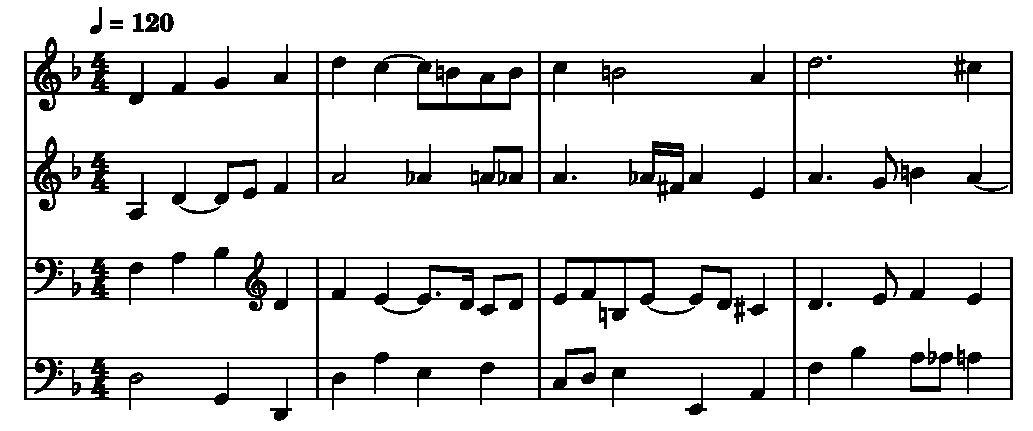
\includegraphics[width=0.9\linewidth]{./img/jsb_7_sheet.pdf}
    \end{center}
    \caption{Fragment chorału J.S. Bacha}\label{fig:jsb_sheet}
\end{figure}
\subsection{WAV i MP3}
WAV \textit{(ang. Waveform Audio Format)} to format plików binarnych, znany z możliwości zapisywania dźwięku bez użycia jakiegokolwiek algorytmu kompresji \cite{wav_specification}. Dzięki temu pliki WAV charakteryzują się najwyższą jakością dźwięku, jednak ich rozmiary są bardzo duże, co może być problematyczne przy przechowywaniu dużych zbiorów danych na dysku. Plik WAV jest najwierniejszą cyfrową reprezentacją dźwięku analogowego. Jego duży rozmiar wynika z faktu, że dźwięk jest zapisywany z częstotliwością 44,1 kHz, czyli w każdej sekundzie w pamięci zapisywane jest 44100 próbek. Format ten został stworzony w 1991 roku i od tego czasu stał się jednym z najbardziej rozpowszechnionych formatów audio, obsługiwanym przez praktycznie każde oprogramowanie do edycji dźwięku. W celu wizualizacji dokonano elektronicznego odtworzenia utworu przedstawionego w postaci nutowej na ilustracji \ref*{fig:jsb_sheet}, co zaowocowało powstaniem fali dźwiękowej, przedstawionej na grafice \ref*{fig:jsb_wav}.

\begin{figure}
    \begin{center}
        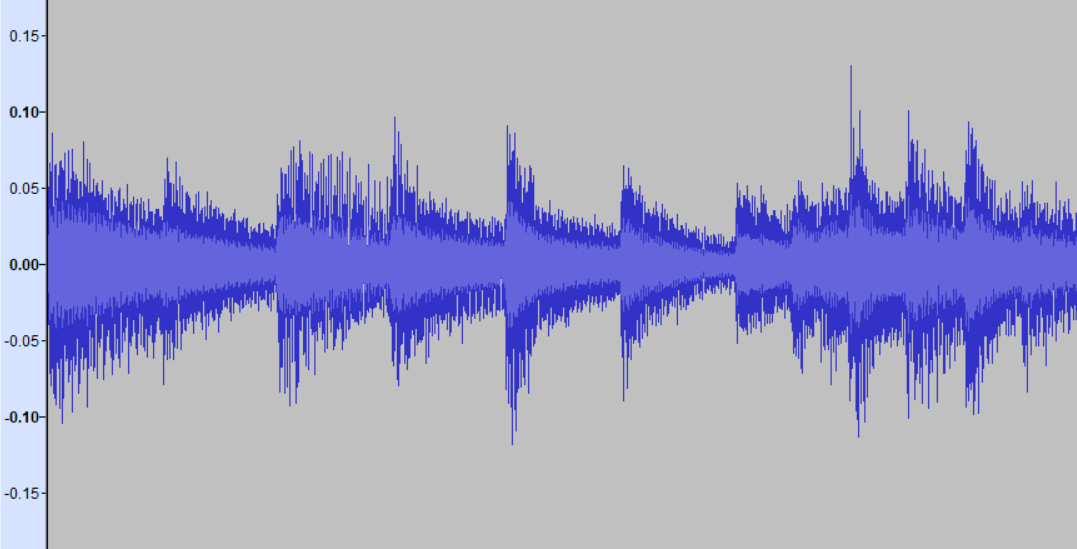
\includegraphics[width=\linewidth]{./img/jsb_wav.png}
    \end{center}
    \caption{Plik \texttt{.wav} otwarty w programie Audacity.}\label{fig:jsb_wav}
\end{figure}

Często nie jest konieczne przechowywanie dźwięku w formacie bezstratnym, ponieważ większość informacji można zachować przy użyciu mniejszej ilości danych. Jednym z najpopularniejszych standardów kodowania stratnego jest format MP3. Kompresja zmniejsza dokładność kodowania i usuwa częstotliwości, które nie są słyszalne dla człowieka. Stratne kodowanie stara się znaleźć równowagę między jakością dźwięku a rozmiarem pliku. W kontekście uczenia maszynowego zmniejszona ilość próbek przy zachowaniu większości informacji jest zjawiskiem pożądanym. Dzięki temu przynajmniej częściowo rozwiązujemy problem związany z ,,przekleństwem wymiarowości'', czyli trudnością w przetwarzaniu danych o bardzo wysokiej liczbie cech (wymiarów). Stratne kodowanie pozwala na efektywniejsze zarządzanie danymi, co może być kluczowe w procesach analitycznych i modelowaniu.

\subsection{Format MIDI}
MIDI \textit{(ang. Musical Instrument Digital Interface)} to standard opisujący protokół komunikacji, interfejs cyfrowy oraz złącze, które umożliwiają połączenie elektronicznych instrumentów, komputerów oraz innych urządzeń muzycznych \cite{midi_specification}. Pojedynczy kabel MIDI może przesyłać informacje na temat szesnastu kanałów jednocześnie, z których każdy może reprezentować inny instrument. Każda interakcja z instrumentem, taka jak naciśnięcie klawisza czy szarpnięcie struny, jest zapisywana jako ,,zdarzenie'' \textit{(event)}, które zawiera takie dane jak znacznik czasu, wysokość dźwięku oraz jego głośność. Dane z urządzeń MIDI są zapisywane w specjalnych plikach z rozszerzeniem \texttt{.mid} lub \texttt{.midi}. Umożliwiają one przechowywanie, rozpowszechnianie oraz edytowanie dźwięków w specjalnie stworzonym do tego oprogramowaniu. Ponieważ plik MIDI nie przechowuje rzeczywistej fali dźwiękowej nagranej przez mikrofon, możliwa jest np. późniejsza zmiana instrumentu, który będzie odtwarzał zapisane dźwięki. Typowym sposobem przedstawienia danych MIDI jest tak zwany \textit{piano roll}, który można porównać do dwuwymiarowego układu współrzędnych, gdzie na osi poziomej reprezentowany jest czas, a oś pionowa przedstawia konkretne dźwięki, pokazane jako klawisze fortepianu. Przykładowe porównanie zapisu MIDI z zapisem nutowym przedstawiono na grafikach \ref*{fig:jsb_pianoroll} oraz \ref*{fig:jsb_sheet}.

\begin{figure}[ht!]
    \begin{center}
        \includegraphics*[width=\linewidth]{./img/piano_roll.png}
    \end{center}
    \caption{Muzyka zapisana w pliku MIDI}\label{fig:jsb_pianoroll}
\end{figure}

Warto zaobserwować, że zapis pliku w formacie MIDI, w porównaniu do zapisu nutowego, umożliwia zdecydowanie większą ekspresję, ponieważ jest to zapis odtworzenia przez artystę pewnego utworu. Pozwala to na ujęcie zdecydowanie więcej emocji jak i osobowości samego muzyka, co może zostać zaobserwowane na przykład przez lekkie przeciąganie pewnych nut lub zmianę głośności ich odegrania. Informacje na temat, tego w jaki sposób odegrać dany utwór (akcenty, głośność nut) mogą zostać zapisane w tradycyjnej notacji, jednak nawet wtedy artysta, może lekko modyfikować zamysł autora utworu.

\subsection{Notacja ABC}
Notacja ABC to system zapisywania nut w formie tekstowej przy użyciu znaków ASCII. Notacja ta pojawiła się w latach 70. XX wieku w celu zapisu i nauki tradycyjnych irlandzkich melodii \cite{abc_history}. W kolejnej dekadzie system ten został rozwinięty przez Chrisa Walshawa, który używał go do zapisywania tradycyjnych melodii, zanim opanował standardowy zachodni zapis nutowy. Walshaw stworzył program \textit{abc2mtex}, który na podstawie notacji ABC generował komendy umożliwiające zapis partytur w formacie \textit{MusicTex}. Obecnie używanym standardem notacji ABC jest wersja z 2011 roku.

\begin{figure}[ht!]
    \begin{minted}[linenos=false]{text}
X:1
Q:1/4=120
V:1
L:1/16
M:4/4
K:C clef=G2
D4F4G4A4|d4c6B2A2B2|c4B8A4|d12^c4|
V:2
L:1/16
M:4/4
K:C clef=G2
A,4D6E2F4|A8^G4A2^G2|A6^G^F^G4E4|A6G2B4A4|
V:3
F,4A,4^A,4D4|F4E7DC2D2|E2F2B,2E4D2^C4|D6E2F4E4|
V:4
L:1/16
M:4/4
K:C clef=F4
D,8G,,4D,,4|D,4A,4E,4F,4|C,2D,2E,4E,,4A,,4|F,4^A,4A,2^G,2A,4|        
\end{minted}
    \caption{Zapis wielu głosów w notacji ABC.}\label{fig:abc_polyphony}
\end{figure}

Rysunek \ref*{fig:abc_polyphony} przedstawia fragment muzyki \ref*{fig:jsb_sheet} zapisany w notacji ABC. Format w dość zwięzły sposób zapisuje partyturę. Poza konkretnymi nutami i rytmem, w tym formacie można zapisać również dodatkowe informacje na temat utworu. W każdej linijce zaczynającej się od znaku A-Z, a następnie dwukropka, znajduje się tak zwane ,,pole informacyjne''. W tych polach można zapisywać takie informacje jak tytuł utworu, metrum oraz wiele innych danych, w tym z jakiego zbioru muzycznego pochodzi utwór lub jaki jest jego tytuł. Wiele z tych informacji powinna zostać usunięta w procesie preprocessingu danych, aby nie zagłuszały tekstem najistotniejszych pól w utworze. Do ważnych pól należą przede wszystkim: domyślna długość nuty (\texttt{L:}), metrum (\texttt{M:}) oraz tonacja w jakiej utwór został napisany (\texttt{K:}). Chociaż model jest w stanie ,,odgadnąć'' te informacje na podstawie dźwięków, ich wyraźne podanie daje modelowi więcej informacji na temat każdej z sekwencji. Dodatkową zaletą podawania tych informacji podczas treningu jest możliwość użycia ich jako początkowej sekwencji, na podstawie której model będzie dalej generował melodię, dzięki czemu można mieć kontrolę nad takimi aspektami jak tonacja i metrum utworu, co pozwala na bardziej precyzyjne kierowanie procesem generowania muzyki.

Notacja ABC wpiera również melodie polifoniczne przy pomocy znaczników \texttt{V:}. Ich ilość nie jest ograniczona, w związku z czym w tym zapisie jest możliwe ujęcie nawet muzyki orkiestrowej. Dość skrajnym przykładem jest zapis drugiej części VII Symfonii Ludwiga van Beethovena, która składa się aż z 19 partii instrumentów \cite{beethoven}.

\subsubsection*{Tokenizacja plików MIDI}\label{sec:REMI}
Tokenizacja to proces przekształcenia danych na mniejsze jednostki zwane tokenami, którymi w kontekście tekstu mogą być słowa, ich fragmenty lub nawet pojedyncze znaki. Tokenizacja jest jednym z pierwszych kroków w analizie tekstu, umożliwiającym dalsze przetwarzanie, takie jak analizę składniową, semantyczną, czy ekstrakcję cech na podstawie zbioru treningowego. Proces ten pomaga w standaryzacji, eliminując niejednoznaczności i ułatwiając dalsze kroki przetwarzania, takie jak stemming czy lematyzację. Algorytmy NLP operujące na tokenach są zazwyczaj bardziej efektywne i łatwiejsze do implementacji. Przetwarzanie mniejszych jednostek tekstu zmniejsza złożoność obliczeniową i pozwala na bardziej precyzyjną analizę \cite*{tokenizacja}. Jednym z głównych powodów tokenizacji jest potrzeba konwersji danych tekstowych na reprezentację numeryczną, która może być przetwarzana przez algorytmy uczenia maszynowego. Korzystając z tej reprezentacji można trenować modele do wykonywania różnych zadań, takich jak klasyfikacja, analiza sentymentu lub generowanie sekwencji tekstowych.

W kontekście plików MIDI proces tokenizacji jest niezbędny, ponieważ format MIDI zawiera skomplikowane struktury i informacje binarne, które są trudne do bezpośredniego wykorzystania przez model. Celem tego procesu jest utworzenie sekwencji tokenów, które będą reprezentować wartości atrybutów nut (wysokość, wartość, czas trwania) lub zdarzenia czasowe zawarte w melodii.

Token może przyjmować jedną z trzech form:
\begin{itemize}
    \item nazwa tokenu - słowna reprezentacja zdarzenia MIDI np. \textit{Pitch\_50}
    \item id - unikalna wartość liczbowa przypisana konkretnemu zdarzeniu
    \item bajt - unikalna wartość liczbowa przypisana podczas treningu tokenizera
\end{itemize}

Nowe słownictwo jest zapisywane w postaci \textit{look up table} łączącej nazwę tokenu z odpowiadającym jej id lub bajtem. Trening tokenizera polega na obliczeniu kodowania gramatykowego np. \textit{byte pair encoding} do postaci tabelarycznej w celu wykorzystania ich w dalszym modelowaniu.

Poza tokenami, które tokenizer tworzy na podstawie pliku MIDI dodaje on również dodatkowe takie jak:
\begin{itemize}
    \item \texttt{PAD} (\textit{padding}) - token używany w przypadku kiedy w partii danych długość sekwencji jest różna; w takim przypadku tym tokenem wydłuża się sekwencje aby wszystkie miały długość najdłuższej
    \item \texttt{BOS} (\textit{beginning of section}) - token oznaczający początek sekwencji
    \item \texttt{EOS} (\textit{end of section}) - token oznaczający koniec sekwencji
\end{itemize}

Istnieje wiele algorytmów tokenizacji MIDI, jednak aby przedstawić mechanizm działania, dokonano analizy popularnego algorytmu \textit{REMI}. \textit{\textbf{RE}vamped \textbf{MI}DI} reprezentuje zdarzenia jako sekwencje tokenów wysokości tonu, dynamiki (głośności), długości oraz czasu trwania poprzez kolejne tokeny. Token taktu oznacza początek nowego taktu, natomiast token pozycji określa miejsce zdarzenia w bieżącym takcie. Porównanie pomiędzy zapisem nutowym a jego reprezentacją w formie tokenów można zaobserwować na ilustracjach \ref*{fig:remi_notes} i \ref*{fig:remi_tokens}. Każda nuta jest reprezentowana przez sekwencję tokenów:
\begin{itemize}
    \item \texttt{Pos} - relatywną pozycję nuty w stosunku do początku taktu zapisaną jako liczba z przedziału 0-31
    \item \texttt{Tempo} - w jakim tempie (\textit{bpm}) nuta została zagrana
    \item \texttt{Pitch} - wysokość dźwięku
    \item \texttt{Vel} - głośność zapisana jako liczba z przedziału 0-127
    \item \texttt{Dur} - długość dźwięku zapisana jako ułamek ćwierćnuty
\end{itemize}
Dodatkowymi tokenami, widocznymi na ilustracji są tokeny \texttt{Bar} odpowiadające za początek taktu oraz \texttt{Rest} kodujące pauzy lub przerwę w muzyce. Wiele algorytmów tokenizacji jest zaimplementowanych w bibliotece MidiTok dla języka Python \cite{miditok2021}.

\begin{figure}[ht!]
    \begin{center}
        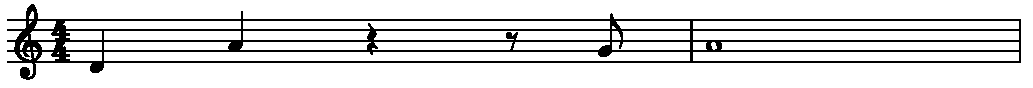
\includegraphics[width=0.9\linewidth]{./img/tokenizer_notes.pdf}
    \end{center}
    \caption{Prosta sekwencja muzyczna}\label{fig:remi_notes}
\end{figure}

\begin{figure}[ht!]
    \begin{center}
        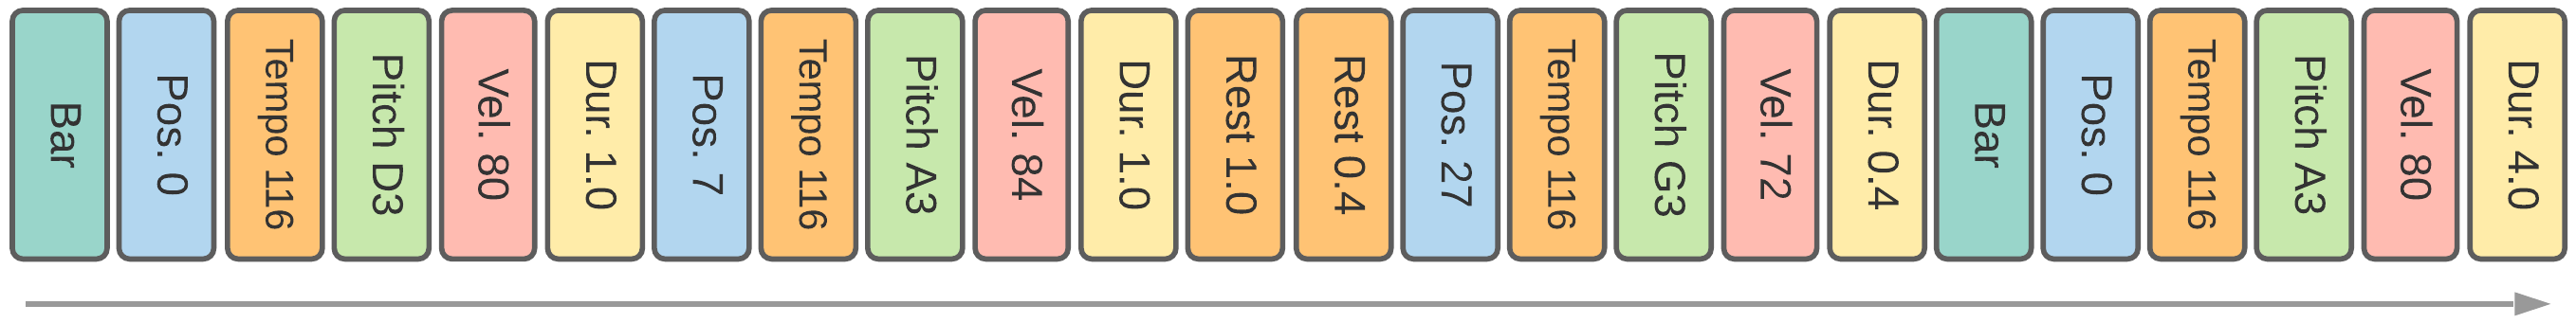
\includegraphics[width=0.9\linewidth]{./img/remi.png}
    \end{center}
    \caption{Reprezentacja muzyki w postaci tokenów}\label{fig:remi_tokens}
\end{figure}

\subsection{Porównanie reprezentacji utworu muzycznego}
W tabeli \ref*{tab:music_diff} zostało przedstawione porównanie zapisu całego utworu, którego fragment przedstawiono na grafice \ref*{fig:jsb_sheet}. Kolumna ,,długość sekwencji'' oznacza liczbę wartości numerycznych opisujących całą sekwencję w danym kodowaniu. W plikach WAV i MP3 są to amplitudy sygnału dźwiękowego, w MIDI długość sekwencji tokenów, a w ABC liczba znaków tekstowych.

\begin{table}[ht!]
    \centering
    \begin{tabular}{|l|l|l|}
        \hline
                      & rozmiar pliku na dysku & długość sekwencji \\ \hline
        \texttt{wav}  & 3971116 B              & 992768            \\ \hline
        \texttt{mp3}  & 360951 B               & 992768            \\ \hline
        \texttt{midi} & 1638 B                 & 740               \\ \hline
        \texttt{abc}  & 953 B                  & 562               \\ \hline
    \end{tabular}
    \caption{Porównanie różnych zapisów muzyki}\label{tab:music_diff}
\end{table}

Jak widać zapis pliku w postaci fali dźwiękowej zajmuje najwięcej miejsca na dysku oraz długość sekwencji, która reprezentuje cały utwór jest największa. W celu uzyskania sekwencji z pliku MIDI został użyty tokenizer REMI o którym jest mowa w rozdziale \ref*{sec:REMI}. Podczas używania innych tokenizatorów długość sekwencji może różnić się nieznacznie pomiędzy nimi. Różnica w rozmiarze na dysku oraz długością sekwencji pomiędzy zapisem MIDI oraz ABC nie jest duża, jednak warto zwrócić uwagę, że gdyby w oryginalnym utworze pojawiły się powtórzenia sekcji melodii, notacja ABC byłaby jeszcze bardziej oszczędna od plików MIDI. Powodem tego jest fakt, że notacja ABC zapisuje bezpośrednio zapis nutowy w postaci tekstowej, którego elementami są znaki repetycji. Są zapisywane znakami \texttt{:|} oraz \texttt{|:}, a w pliku MIDI cała powtarzana sekwencja musi zostać ponownie odegrana.

Do głównych zalet plików MIDI należy ich wszechstronność. Nie są one ograniczone do sztywno określonego rytmu w postaci ćwierćnut, ósemek czy szesnastek, jak w innych notacjach muzycznych, co daje zdecydowanie większe możliwości ekspresji. Dodatkowo, przy użyciu narzędzi komputerowych, bardzo łatwo można zamienić dowolny zapis nutowy (np. MusicXML lub ABC) na plik MIDI. Niestety, w drugą stronę, czyli konwersja pliku MIDI na zapis nutowy, jest znacznie trudniejsza, głównie z powodu nieokreślonego rytmu. Istnieją narzędzia, takie jak MuseScore, które potrafią wygenerować partyturę z pliku MIDI, jednak skuteczność tych narzędzi nie zawsze jest wysoka, zwłaszcza w przypadku bardziej skomplikowanych utworów, gdzie rytm i artykulacja mogą być trudne do dokładnego oszacowania. Mimo tych wyzwań, pliki MIDI pozostają niezwykle użyteczne w zastosowaniach muzycznych, od tworzenia i edytowania muzyki po jej analizę i odtwarzanie.

Zapis pliku w postaci fali dźwiękowej niesie ze sobą wiele wad, jednak jest to często jedyne rozwiązanie, aby zebrać dużą ilość danych szczególnie w przypadku muzyki nowoczesnej, kiedy twórcy nie udostępniają zazwyczaj plików MIDI ani zapisu nutowego, na podstawie którego powstał dany utwór. Z tego powodu praca z plikami MP3 lub czasochłonna translacja muzyki na inny format jest często konieczna.

Zaletą plików dźwiękowych w zapisie cyfrowym jest dostęp do potencjalnie istniejącego zapisu odśpiewanego tekstu. Pomimo że notacja ABC pozwala na zapis tekstu w znaczniku \texttt{W:}, jest to jedynie zapis słowny, a nie faktyczne odśpiewanie. W związku z tym pliki WAV są bardziej odpowiednie do próby replikacji czyjegoś głosu, ponieważ zawierają rzeczywisty zapis audio, który można analizować i przetwarzać.

Główną zaletą plików ABC jest ich tekstowa reprezentacja notacji muzycznej. Z tego powodu nie wymagaja one wiedzy na temat struktury, budowy oraz standardów plików np. MIDI aby zacząć z nimi pracować. Ponieważ notacja ABC jest tekstowa, można ją łatwo integrować z narzędziami do przetwarzania tekstu. Zwięzłość zapisu jest również przyczyną, dla której model uczenia maszynowego może być mniejszy w związku z mniejszą ilością tokenów w sekwencji, na podstawie której model się uczy. Zapis w postaci tekstu pozwala na bardzo proste dodanie pewnych dodatkowych danych, które można policzyć w etapie procesowania danych. Podejście takie zostało zaproponowane w modelu \textit{Tunesformer} \cite{tunesformer}, który wziął przykład z artykułu \cite{keskarCTRL2019}, w którym autorzy dodawali do korpusu treningowego danych tekstowych takie znaczniki jak \textit{Books}, \textit{Horror}, \textit{Relationships}, \textit{Legal}. Oznaczenia te były podawane na początku pytania podawanego dla modelu, przez co model miał w jasny sposób podane w jakim stylu powinien udzielić odpowiedzi. W przypadku muzyki w zapisie ABC zostały wprowadzone nowe kody kontrolne.

\begin{itemize}
    \item \texttt{S:} - Reprezentuje liczbę sekcji w całym utworze. Znacznik jest \textcolor{blue}{łatwy} do policzenia ponieważ początek i koniec taktu jest jawnie oznaczany przy pomocy symboli \texttt{[|}, \texttt{||}, \texttt{|]}, \texttt{|:}, \texttt{::} i \texttt{:|}
    \item \texttt{B:} - Oznacza liczbę taktów w danej sekcji czyli zlicza tylko wystąpienia znaku \texttt{|}.
    \item \texttt{E:} - Kontroluje poziom podobieństwa pomiędzy dwoma następującymi po sobie sekcjami. W związku z tym, że zapis melodii jest w postaci tekstu, można policzyć podobieństwo używając odległości Levenshteina \textcolor{blue}{według} wzoru:
          \begin{equation}
              E(c,p) = 1 - \dfrac{lev(c, p)}{\text{max}(|c|, |p|)}
          \end{equation}
          gdzie $c$ oraz $p$ to następujące po sobie sekwencje, a $|c|$, $|p|$ to ich długości.
\end{itemize}

Policzone kody wraz z ich odpowiednim oznaczeniem dodawane są do pliku tekstowego, który zapisuje notacje. Dodanie ich nie sprawia, że notacja staje się nieprawidłowa. Tak samo jak w przypadku \textcolor{blue}{znaczników}, które opisują elementy zapisu jak tonacja czy metrum, służą one nam oraz modelowi jako wskazówki, którymi powinien się sugerować podczas generowania muzyki.

\section{Zbiory danych}

\subsection{Johann Sebastian Bach Chorales}
\textit{JSB Chorales} \cite{bachchorales} to zbiór krótkich, czterogłosowych utworów pierwotnie skomponowanych przez Johanna Sebastiana Bacha w XVIII wieku. Napisał je biorąc wcześniej istniejące melodie ze współczesnych mu hymnów luterańskich, a następnie harmonizując je w celu stworzenia pozostałych trzech głosów. Zbiór danych zawiera 382 takich chorałów. Dodatkowo ich rytm został znormalizowany przez co najmniejszą długością nuty jest szesnastka. Dzięki temu uproszczeniu zbiór jest bardzo łatwo konwertowalny do dowolnego \textcolor{blue}{formatu} zapisu które zostały zaprezentowane na grafikach \ref*{fig:jsb_sheet}, \ref*{fig:jsb_pianoroll}, \ref*{fig:abc_polyphony}.

Dodatkową zaletą takiego rytmu jest możliwość pominięcia użycia tokenizera MIDI, ponieważ wiedząc że rytm jest stały i wyznaczony przez szesnastkę, można użyć naiwnego podejścia i zapisać każdy głos jako wektor, którego wartościami są wysokości \textcolor{blue}{kolejno brzmiących dźwięków.} Po złożeniu wektorów w macierz 4 $\times$ (długość utworu) można przejść do analizy. Wadą tego podejścia jest możliwość wystąpienia macierzy rzadkich, które często stanowią problem dla algorytmów uczenia maszynowego \cite*{sparse_matrix}, jednak w tym zbiorze ten problem nie wystepuje.

\subsection{The MAESTRO v3.0}
Zbiór danych MAESTRO \cite{maestrov3} powstał w współpracy z \textit{Minnesota International Piano-e-Competition}, czyli międzynarodowym konkursem pianistycznym. Litera \textit{e} w nazwie odnosi się do fortepianów Yamaha Disklavier używanych podczas konkursu, które poza tradycyjną funkcjonalnością są obudowane elektronicznymi sensorami, które pozwalają między innymi zapis odegranej muzyki w formacie MIDI. Z tego powodu organizacja Magenta działająca wewnątrz Google użyła zapisu melodii z wielu edycji konkursu aby stworzyć \textcolor{blue}{zbiór danych} zawierający około 200 godzin muzyki fortepianowej. W tych 200 godzinach znajduje się 1276 \textcolor{blue}{wystąpień pianistycznych} w skład których wchodzi ponad 7 milionów nut. Dwa rodzaje zbioru jakie można pobrać to zbiór w wersji WAV oraz MIDI. Pierwszy, z powodów omawianych we wcześniejszych częściach pracy, zajmuje aż 122 GB, natomiast wersja MIDI zajmuje tylko 81 MB.
% MIDI-Unprocessed_08_R1_2009_01-04_ORIG_MID--AUDIO_08_R1_2009_08_R1_2009_01_WAV.midi
\begin{figure}[ht!]
    \begin{center}
        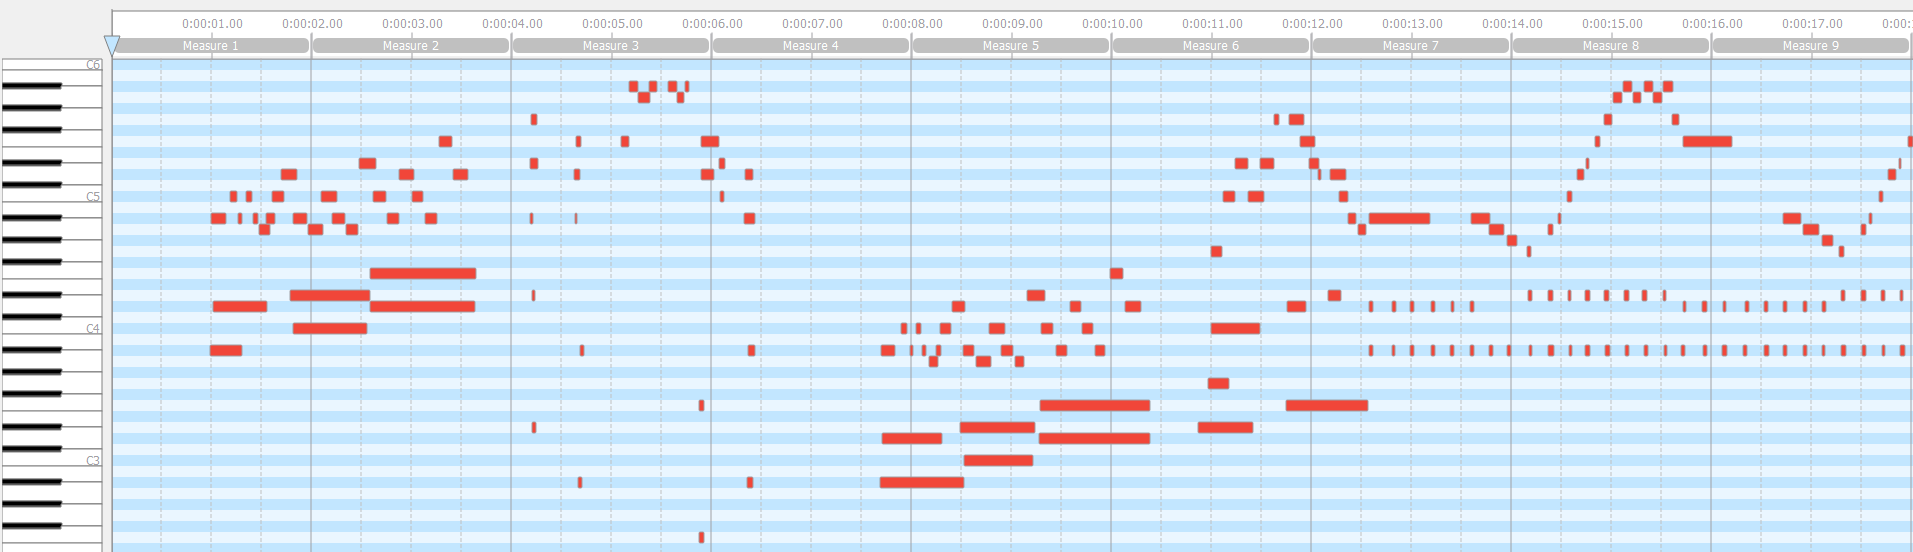
\includegraphics[width=0.9\linewidth]{./img/maestro_1.png}
    \end{center}
    \caption{{Przykład utworu pochodzącego ze zbioru MAESTRO.}}\label{fig:maestro_midi}
\end{figure}

Porównując zapis prostego utworu widoczny na grafice \ref*{fig:jsb_pianoroll} z tym na grafice \ref*{fig:maestro_midi} osoby nawet nie znające się na muzyce są w stanie wywnioskować że jest to utwór bardziej złożony. Jak widać odegrane nuty często nie padają na sztywno określone rozpoczęcie taktu, przez co potencjalnie wygenerowana muzyka na podstawie tego zbioru będzie wydawała się bardziej ekspresyjna oraz ,,ludzka''.

\subsection{IrishMAN}
Zbiór danych IrishMAN (\textit{ang. Irish Massive ABC Notation}) \cite{irishman} zawiera 216,248 fragmentów tradycyjnych irlandzkich melodii. Pochodzą one ze stron takich jak \texttt{thesession.org} oraz \texttt{abcnotation.org}, które znane są z udostępniania tradycyjnej muzyki w różnych formatach. Aby zapewnić jednolitość formatowania najpierw wszystkie utwory zostały przekonwertowane do notacji MusicXML, a nastepnie do notacji ABC. Istnieją bliźniacze zbiory IrishMAN-MIDI oraz IrishMAN-XML, które zawierają te same utwory jednak zapisane w odpowiadających ich \textcolor{blue}{nazwom} formatach. Wszystkie fragmenty muzyki należą do domeny publicznej, w związku z czym można korzystać z tych melodii bez obaw o łamanie praw autorskich. Zbiór jest o tyle ciekawy że zawiera w sobie muzykę jedno, jak i wielogłosową. Autorzy zbioru udostępnili również skrypty napisane w języku Python przy pomocy których, można samemu stworzyć własne zbiory danych na podstawie swoich plików ABC lub MusicXML. Jest to również jeden z niewielu zbiorów, który udostępnia te same fragmenty muzyki w różnych formatach, przez co nadaje się on wyjątkowo dobrze do porównywania różnych algorytmów generatywnych.

\begin{figure}[ht!]
    %valid/98.mid
    \begin{center}
        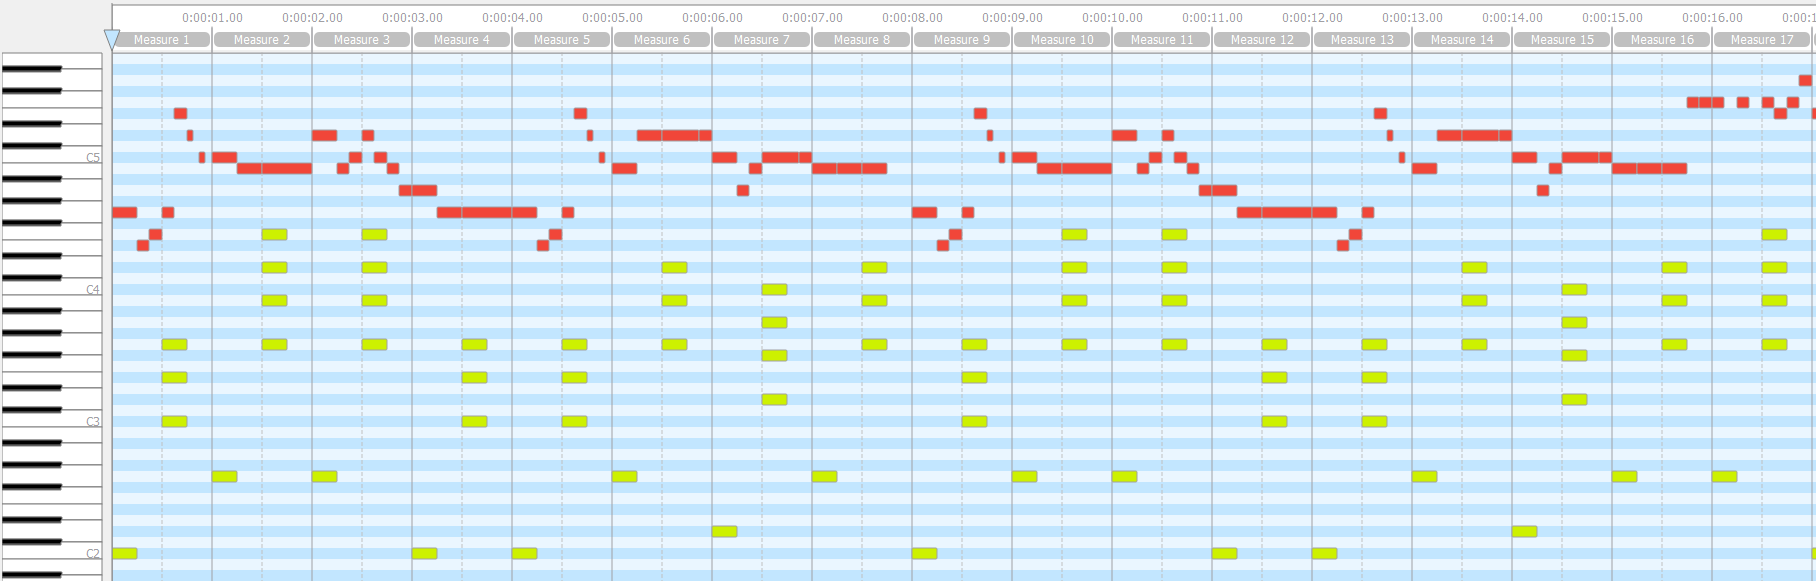
\includegraphics[width=0.9\linewidth]{./img/irishman_midi.png}
    \end{center}
    \caption{Przykład wielogłosowego fragmentu ze zbioru IrishMAN.}\label{fig:irish_midi}
\end{figure}

\section{Architektura transformera}
\subsection{Sieci RNN}
Pierwszymi próbami użycia sieci neuronowych w przetwarzaniu sekwencji było użycie rekurencyjnych sieci neuronowych. Architektura ich była prosta i dodawała ona pętlę w taki sposób, aby wartości wynikowe mogły być przekazywane pomiędzy krokami. Rysunek \ref*{fig:rnn_scheme} przedstawia fragment sieci oraz jej rozwinięcie \cite{Understanding_lstm}.
\begin{figure}[ht!]
    \begin{center}
        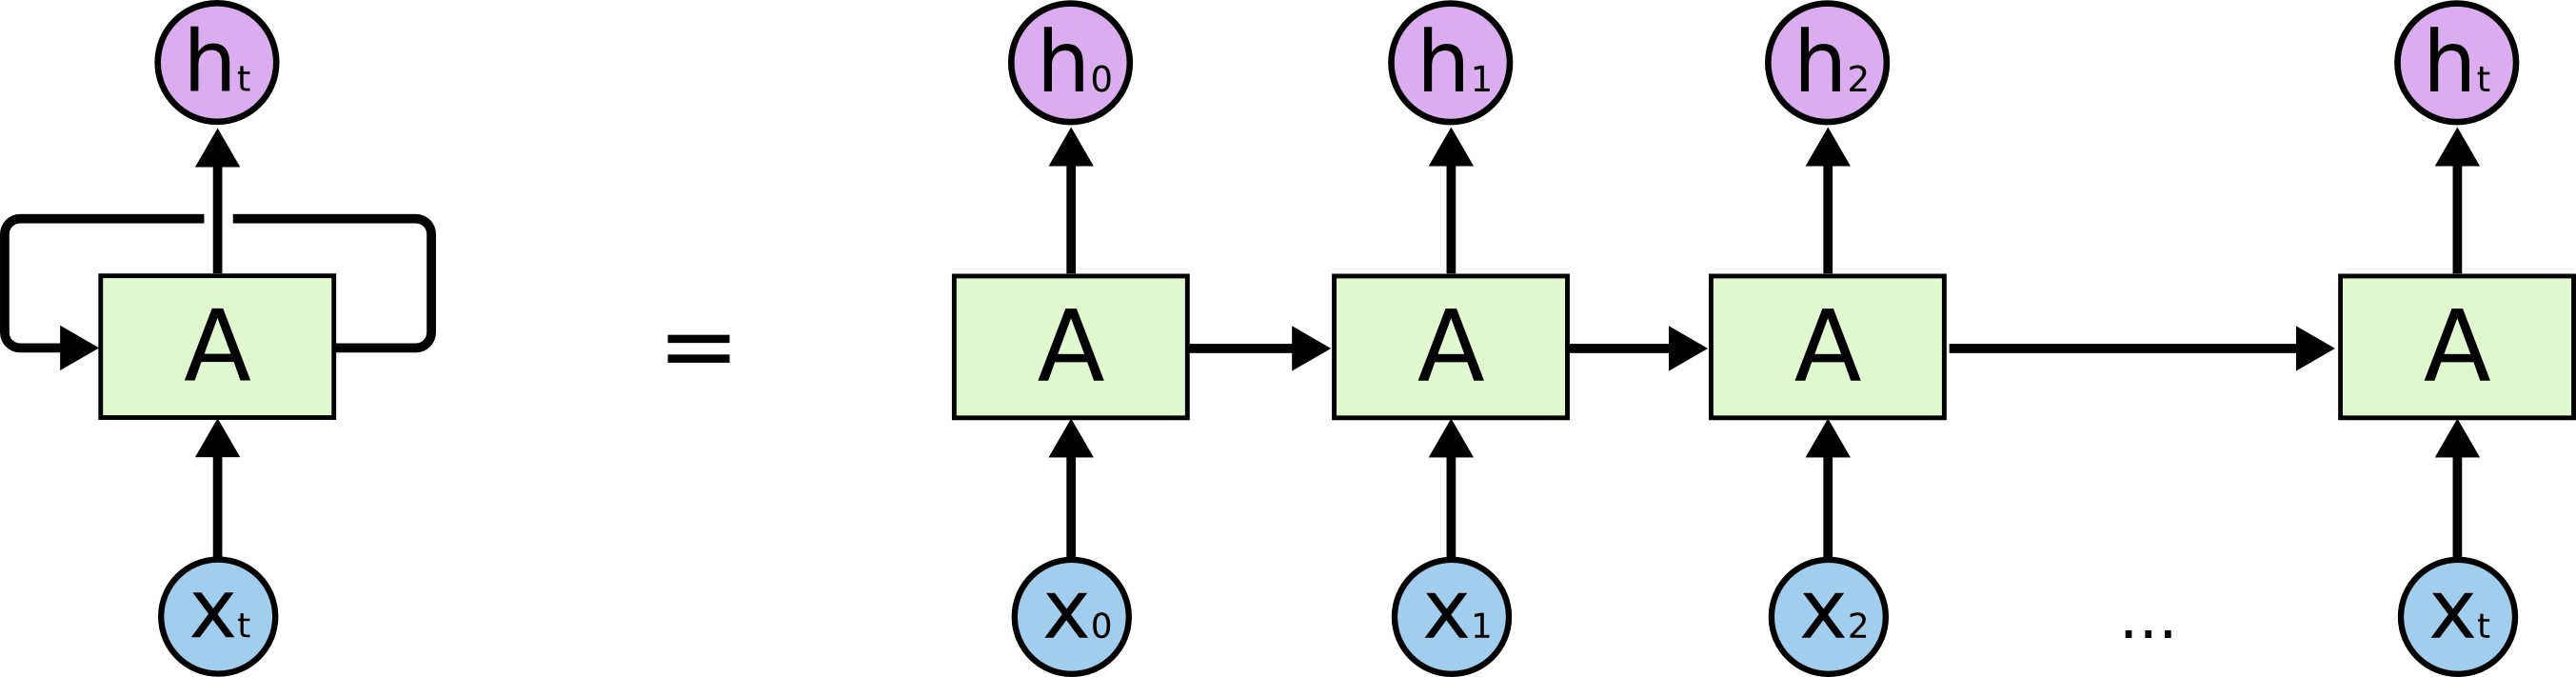
\includegraphics[width=0.7\linewidth]{./img/rnn_scheme.png}
    \end{center}
    \caption{Schemat budowy fragmentu sieci RNN.}\label{fig:rnn_scheme}
\end{figure}

Prezentowane podejście jest dość proste, jednak niesie ze sobą pewne problemy.

Pierwszym z nich jest brak selekcji, które informacje są rzeczywiście istotne w danym kontekście, a które nie. W zadaniu przewidywania kolejnego słowa np. dla zdania ,,Kupiłem zegarek na \textit{rękę}'' nie jest wymagany żaden dodatkowy kontekst, a odległość pomiedzy ważnymi informacjami jest mała, jednak w zdaniu ,,Rok temu ukończyłem kurs lotnika ... Teraz staram się o licencję \textit{pilota}'' wymagane jest szersze spojrzenie na całą strukturę wypowiedzi i ,,przypomnienie'' informacji z początku zdania. W przypadku muzyki sytuacja wygląda dokładnie tak samo. Przykładowo, aby rozwiązać akord dysonansowy na konsonansowy lub dominantowy na tonikę, wymagana jest jedynie informacja na temat ich dzięków, tak aby dobrać odpowiedni nowy akord, jednak jeśli w muzyce przewija się pewien temat, to wymagane jest zachowanie informacji w sieci, w jakich momentach się on pojawia, aby móc dodać go w odpowiednie miejsce. W teorii zwyczajna sieć rekurencyjna jest zdolna do zapamiętywania długich zależności, jednak w praktyce jest to bardzo rzadko osiągalne.

Dodatkowym problemem podczas treningu modeli jest problem zanikającego gradientu. Równanie \ref*{equ:gradient} przedstawia obliczenia przeprowadzane w celu wyznaczenia konkretnego stanu ukrytego $h_i$.

\begin{equation} 
    \begin{aligned}
         & h_{i+1}=Wh_i+Zx_i  \\
         & h_1=Wh_0+Zx_1  \\
         & h_2=W^2h_0+WZx_1+Zx_2 \\
         & \vdots \\
         & h_N = W^Nh_0+W^{N-1}Zx_1 +\dots + Zx_N\\
    \end{aligned}
    \label{equ:gradient}
\end{equation}
\textcolor{blue}{W powyższym równaniu wartość $N$ oznacza długość okna kontekstowego na którym operuje model, $W$ macierz wag z obecnego kroku, a $Z$ jest wagami z kroku poprzedniego. Aby obliczyć stan ukryty, na podstawie którego zostanie dokonana dalsza predykcja, należy policzyć każdy poprzedni stan zaczynając od pierwszego. Aby uchwycić odpowiedni kontekst fragmentu testu długość okna kontekstowego powinna być maksymalnie długa. Z tego powodu podczas obliczeń macierz wag $W$ będzie podnoszona do bardzo wysokiej potęgi przez co jej wartości poniżej $1$ będą zanikać do $0$ (zanikający gradient), a te będące powyżej $1$ będą dążyły do nieskończoności (eksplodujący gradient). W przypadku drugiego problemu istnieją metody regularyzacyjne takie jak ,,ucinanie gradientu'' (\textit{gradient clipping}), które starają się go rozwiązać \cite*{deeplearning_book}. W przypadku zanikającego gradientu można zastosować normalizację pakietu danych (\textit{batch normalization}), która jednak nie zawsze rozwiązuje tan problem \cite*{batch_norm}.}

\subsection{LSTM}
Aby rozwiązać omawiane problemy sieci rekurencyjnych została zaproponowana architektura sieci nazwana \textit{Long Short Term Memory} \cite{lstm_og}. Ich budowa pozwala na długofalowe zapamiętywanie i przekazywanie informacji. Warstwy LSTM są zazwyczaj łączone między sobą co pozytywnie wpływa na działanie sieci.


\textcolor{blue}{Komórka LSTM zwraca dwa wektory. Pierwszy, stan ukryty (\textit{hidden state}), który jest wektorem przechowującym informacje o bieżącym stanie sieci w danym kroku. Wartości są aktualizowane przy każdym kroku czasowym na podstawie nowych danych wejściowych oraz poprzedniego stanu ukrytego. Reprezentuje krótkoterminowe informacje w sekwencji, które są potrzebne do generowania odpowiedzi na bieżącym etapie. Stan komórki (\textit{cell state}), to dodatkowy wektor, który przechowuje informacje długofalowe, czyli takie, które nie wynikają bezpośrednio z niedalekich poprzednich komórek. Jego struktura umożliwia łatwe przekazywanie informacji w dłuższej perspektywie, co jest kluczowe w zadaniach wymagających pamięci długoterminowej. Stan komórki jest modyfikowany za pomocą trzech bramek: bramki wejścia (\textit{input gate}), bramki zapomnienia (\textit{forget gate}) oraz bramki wyjścia (\textit{output gate}).}

\begin{figure}[ht!]
    \begin{center}
        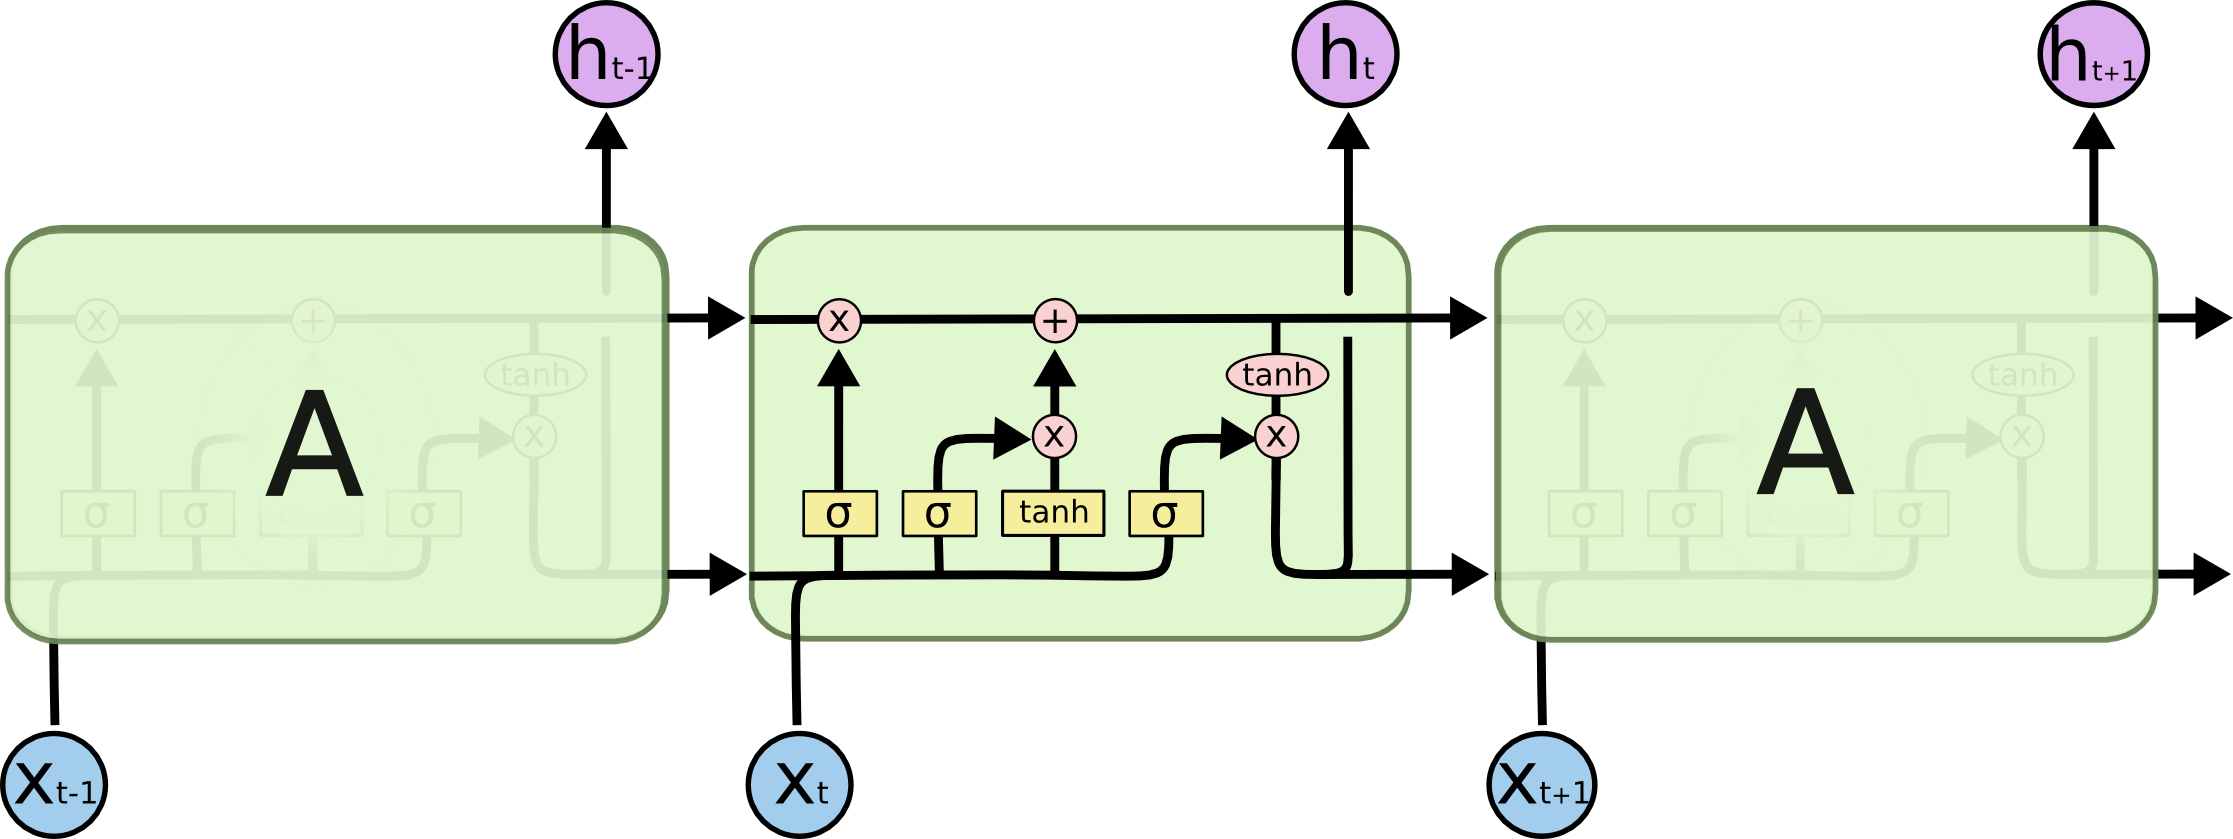
\includegraphics[width=0.6\linewidth]{./img/LSTM3-chain.png}
    \end{center}
    \caption{Komórki LSTM połączone między sobą.}\label{fig:lstm_chain}
\end{figure}

\textcolor{blue}{Główną częścią budowy komórki jest górna część reprezentowana przez prostą, biegnącą przez całą jej długość strzałkę na ilustracji \ref*{fig:lstm_chain} \cite{Understanding_lstm}, która posiadając jedynie proste operacje liniowe przekazuje stany ukryte z jednej części do drugiej. Dolna część komórki zawiera wcześniej wspomniane bramki, które kontrolują, które informacje są ważne i mają być zachowane, a które można zignorować. Są one zbudowane z warstw sigmoidalnych oznaczonych na grafice literami $\sigma$. Wartościami zwrotnymi \textcolor{blue}{bramek} jest liczba pomiędzy $0$ a $1$, gdzie mała wartość znaczy niską, a wysoka dużą ważność informacji.} 

Architektura takiego modelu sprawia, że jest on o wiele mniej podatny na problem zanikającego gradientu, jednak jest to sytuacja, która niestety może nadal występować \cite{vanishing_gradient}. \textcolor{blue}{Dodatkową wadą modelu LSTM jak i klasycznego RNN jest ich wysoka złożoność treningu, która występuje z powodu konieczności użycia specjalnego wariantu algorytmu wstecznej propagacji błędu nazywanego ,,wsteczną propagacją błędu w czasie'' (\textit{backpropagation through time}), która generuje rozwinięcie sieci rekurencyjnej na wiele kroków czasowych, tworząc rozłożony na warstwy graf obliczeń. Następnie stosowana jest tradycyjna propagacja wsteczna do obliczenia gradientów błędów w stosunku do wag sieci na każdym kroku czasowym. Gradienty te są sumowane, a wagi są aktualizowane w celu minimalizacji błędu predykcji w całej sekwencji, umożliwiając sieci lepsze dopasowanie do danych sekwencyjnych.}

Istnieje kilka wariantów LSTM-ów np. dwukierunkowe LSTM, które pozwalają aby informacja przepływa w dwóch kierunkach na raz a nie tylko z lewej strony do prawej \cite{bi_lstm}. Użycie takich modeli poprawia skuteczność i wyniki w stosunku do klasycznego modelu, jednak problemy z ich treningiem dalej pozostają lub nawet stają się jeszcze większe.

\subsection{Algorytm uwagi (ang. \textit{attention})}
\label{sec:attention}
Mechanizm uwagi (\textit{ang. attention}) został zaproponowany w przełomowym artykule \\,,\textit{Attention is All You Need}'' \cite{attention}. Algorytm ten działa w ustalonym oknie kontekstowym \\ (\textit{ang. context window}), w którym przydziela każdemu słowu wagę reprezentującą jego ważność w danym kontekście. Metoda ta imituje sposób w jaki człowiek, czytając na przykład książkę, skupia się na różnych fragmentach tekstu w danym momencie, interpretując dane słowa w kontekście innych, już przeczytanych oraz tych, które zostaną przeczytane za chwilę. Mechanizm uwagi został opracowany, aby rozwiązać problem występujący w rekurencyjnych sieciach neuronowych, gdzie ,,ważność'' słowa była tym większa, im bliżej końca sekwencji się ono znajdowało, co sprawiało, że modele często ignorowały informacje znajdujące się \\ na początku okna kontekstowego. Mechanizm uwagi został zaprojektowany tak, aby identyfikować najwyższe korelacje między słowami w zdaniu, zakładając, że \textcolor{blue}{zostaną one wykryte na podstawie} zbioru treningowego. Korelacja ta jest przechwytywana w wagach neuronów poprzez propagację wsteczną albo z samonadzorowanego szkolenia wstępnego, albo z nadzorowanego \textcolor{blue}{dostrajania}. Algorytm działa na wartościach liczbowych, więc przed analizą, każda sekwencja musi zostać \textcolor{blue}{zakodowana} (\textit{embedded}) \textcolor{blue}{w postaci} wektora o określonej długości.

W kontekście muzyki problem zanikania kontekstu jest jeszcze bardziej widoczny niż \\ w tradycyjnych problemach przetwarzania języka naturalnego, ponieważ na początku zapisu nutowego znajdują się kluczowe dla niego informacje, takie jak metrum czy tonacja utworu zapisana za pomocą krzyżyków lub bemoli. Z tego powodu model, analizując dalsze części sekwencji, może ignorować te istotne elementy.

Podstawowa wersja algorytmu nazywana jest \textit{self-attention} lub \textit{scaled dot-product attention} ponieważ sekwencja ,,zwraca uwagę'' na samą siebie, czyli innymi słowy każdy token\\  w sekwencji jest rozważany z każdym innym poza sobą. Zależności pomiędzy słowami\\ w mechanizmie uwagi można przedstawić jako graf pełny skierowany, gdzie wierzchołkami\\ są poszczególne słowa lub inne tokeny z okna czasowego, a krawędziami są wartości określające, jak istotne dla danego słowa są wszystkie inne. Jest to zdecydowanie lepsze podejście niż to z \textcolor{blue}{RNN} lub LSTM-ów, gdzie zależności są przekazywane jedynie w wektorze, który kompresuje kontekst ze wszystkich poprzednich słów. Dzięki temu mechanizm uwagi pozwala na bardziej dynamiczną kontrolę i monitorowanie, jak zależności pomiędzy tokenami formują się podczas treningu.


\begin{figure}[ht!]
    \centering
    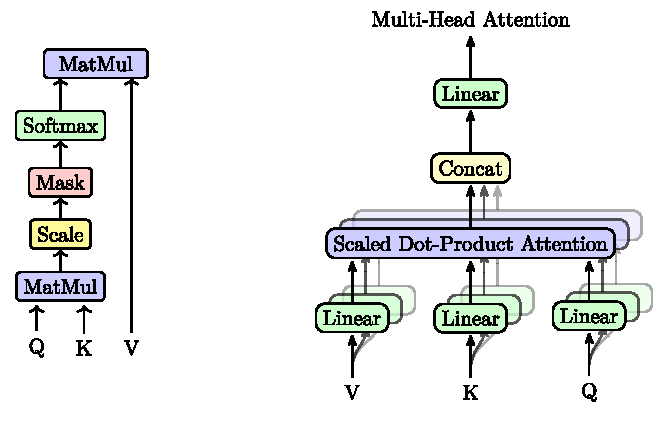
\includegraphics[width=0.7\linewidth]{./img/attention_heads.pdf}
    \caption{Schemat mechanizmu uwagi oraz ich kilkukrotne złożenie.}\label{fig:attention_heads}
\end{figure}

Przedstawione na rysunku \ref*{fig:attention_heads} wartości $K$ (Key), $V$ (Value) i $Q$ (Query) w mechanizmie \textit{self-attention} są uzyskiwane przez przemnożenie danych wejściowych i \textcolor{blue}{odpowiadających} im nauczonych macierzy wag. Dla każdego elementu sekwencji (reprezentowanego przez jego zapytanie $Q$), obliczane jest podobieństwo \textcolor{blue}{do każdego innego elementu sekwencji} (\textcolor{blue}{reprezentowanego} przez klucze $K$). Najczęściej używa się iloczynu skalarnego, który jest normalizowany przez wymiar osadzonego wektora ($d_k$) aby uzyskać współczynniki uwagi a następnie, aby wartości sumowały się do jedynki używana jest funkcja softmax. Ten krok można rozumieć jako tworzenie \textcolor{blue}{słownika w którym} kluczami są poszczególne tokeny, a odpowiadającymi im wartościami \textcolor{blue}{są miary ważności} w całej sekwencji. Każda wartość $V$ jest ważona przez współczynniki uwagi obliczone w poprzednim kroku, co pozwala modelowi skupić się na najistotniejszych elementach sekwencji. Cały ten złożony proces sprowadza się do jednego równania zapisanego w \ref*{equ:attention}. W algorytmie można dodać opcjonalną maskę, która umożliwia zasłonięcie niektórych wartości uwagi, dzięki czemu te tokeny nie będą na siebie wpływać. Prosty schemat tego algorytmu został pokazany na lewej stronie grafiki \ref*{fig:attention_heads}.

\begin{equation}
    \text{Attention}(Q, K, V) = \text{softmax}\left(\dfrac{QK^T}{\sqrt{d_k}}\right)V
    \label{equ:attention}
\end{equation}

Aby zeskalować model i zwiększyć liczbę jego parametrów w celu użycia go do bardziej zaawansowanych celów, można użyć algorytmu \textit{multi-headed attention}. Jest to kilka warstw uwagi, przed wejściem do których znajduja się warstwy liniowe. Wartości po wyjściu z algorytmu \textit{attention} są konkatenowane, a następnie ponownie przetwarzane przez warstwę liniową. Tym sposobem, zamiast tylko jednej instancji mechanizmu uwagi, model może korzystać z wielu. Schemat takiego podejścia pokazano na prawej stronie grafiki \ref*{fig:attention_heads}.

\subsection{Transformer}
Wraz z wprowadzeniem algorytmu uwagi, w tym samym artykule został zaproponowana architektura modelu uczenia maszynowego wykorzystująca \textit{multi-headed attention}. Cały model składa się z dwóch części nazwanych enkoderem oraz dekoderem.

\begin{figure}[!ht]
    \begin{center}
        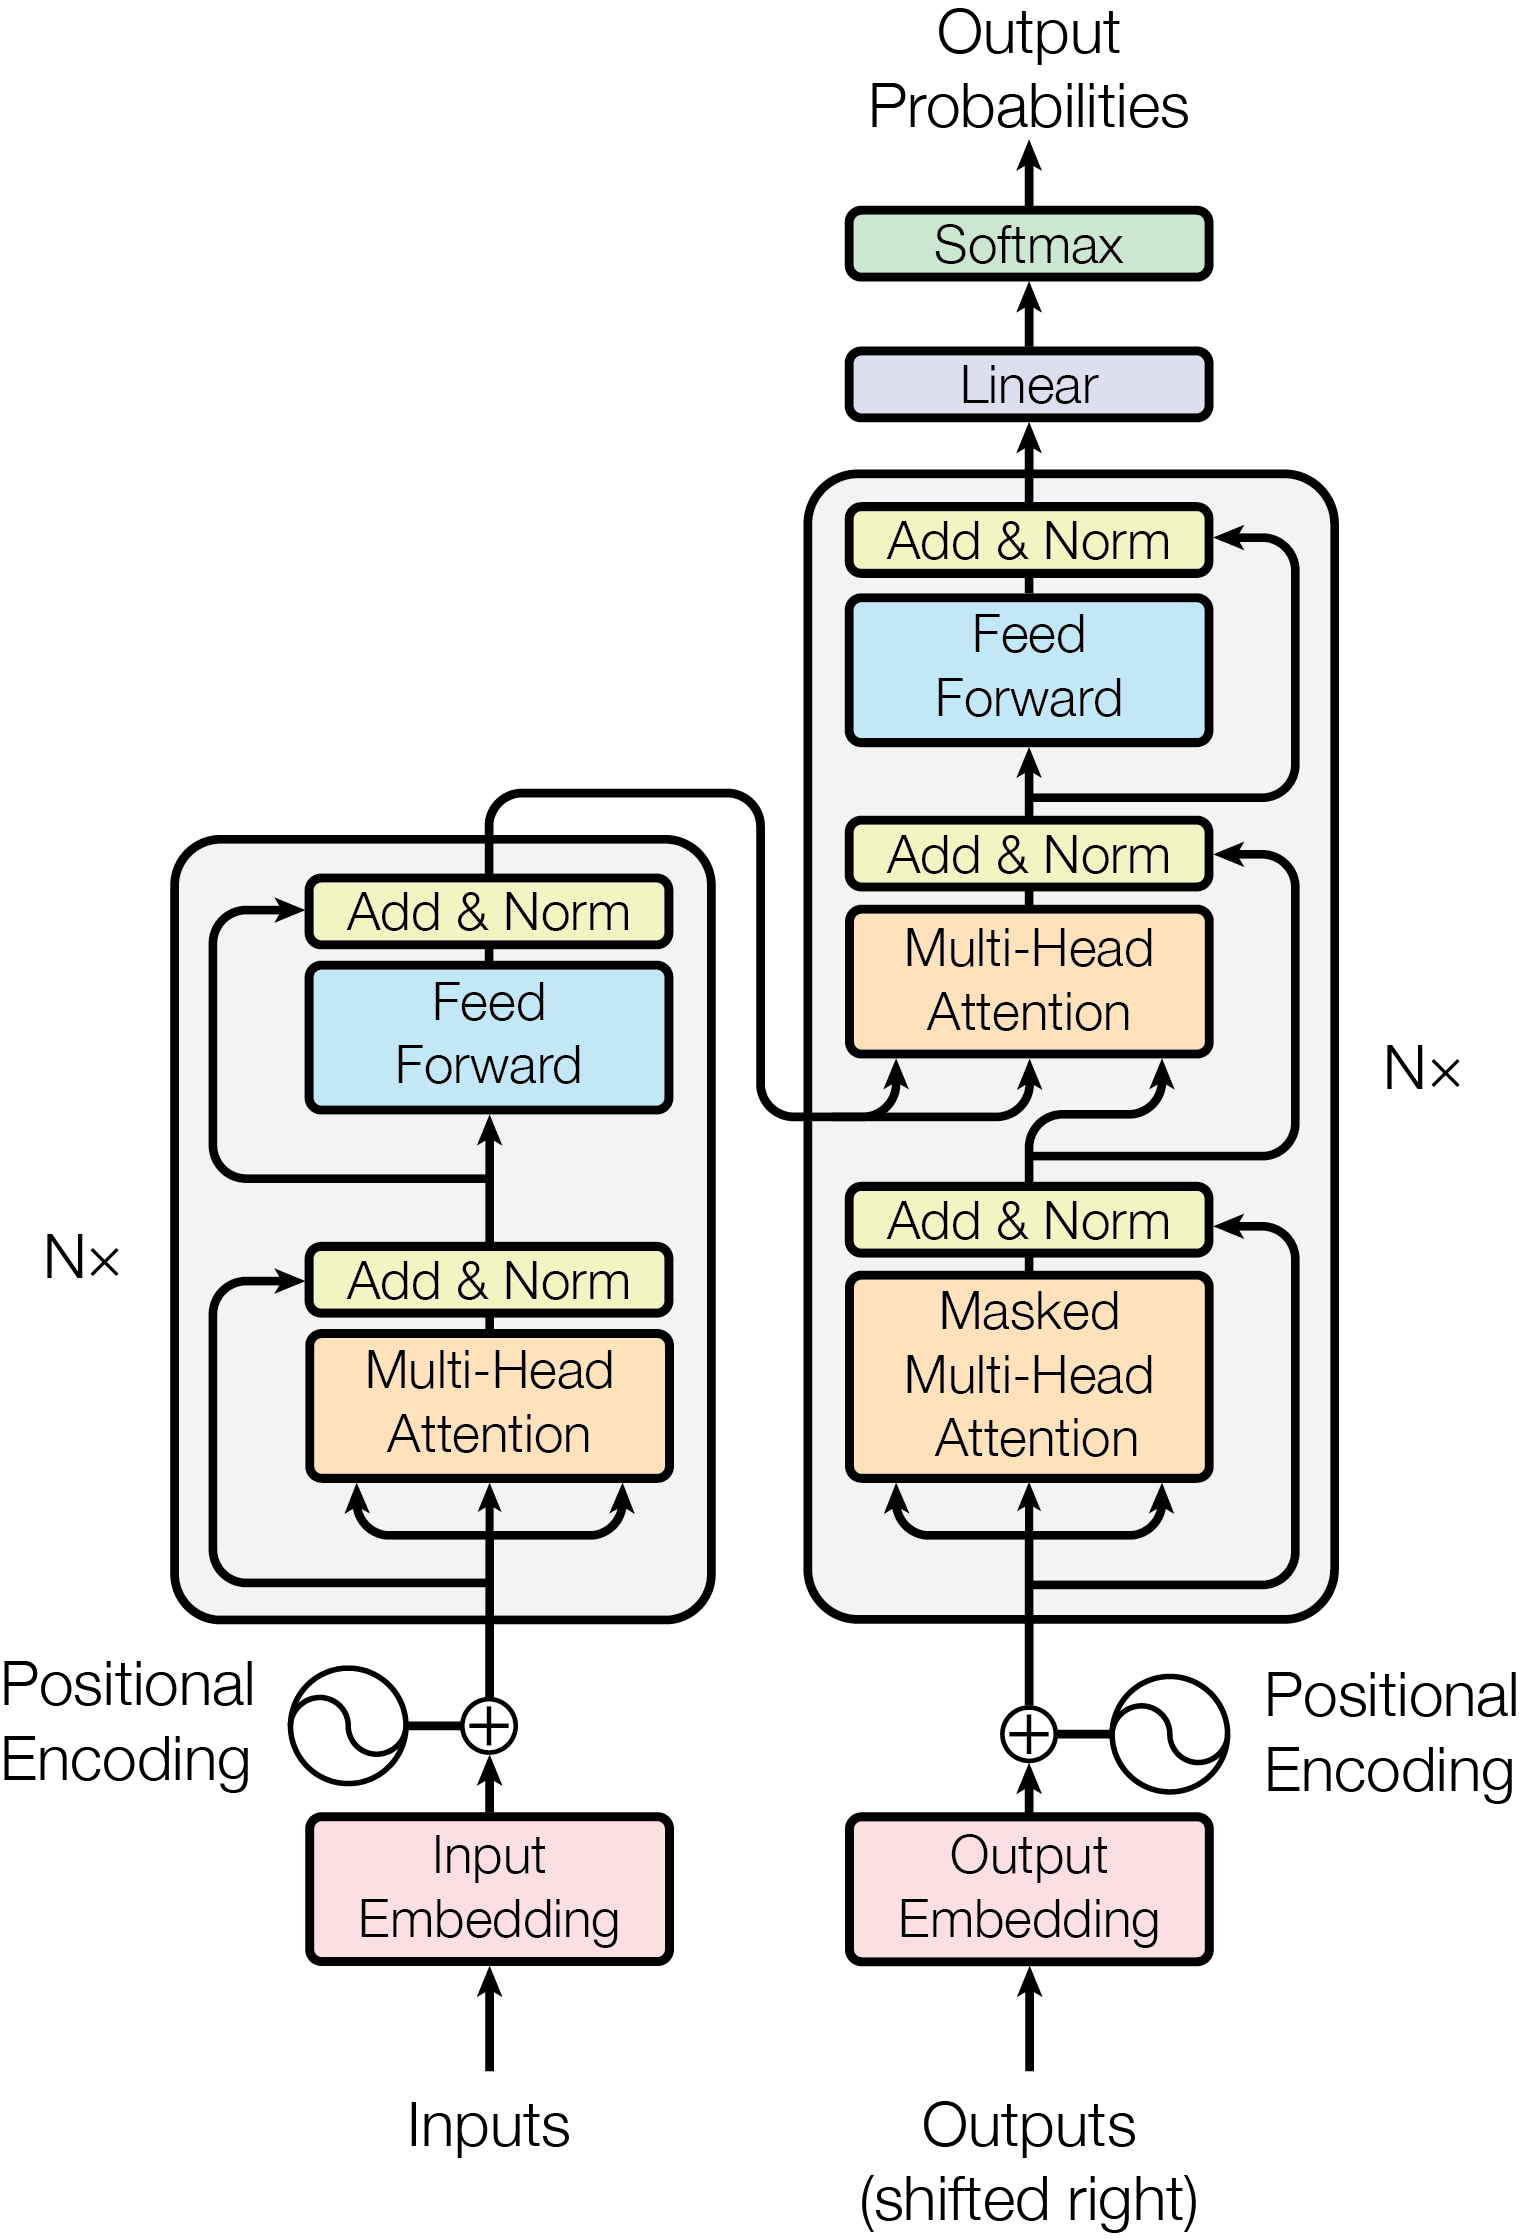
\includegraphics[width=0.7\linewidth]{img/transformer1}
    \end{center}
    \caption{Schemat transformera.}
    \label{fig:transformer1}
\end{figure}

\subsubsection*{Enkoder}
Zadaniem enkodera jest zapoznanie się z całym korpusem tekstu i przekazanie zebranych informacji do dekodera. Mechanizm samo-uwagi \textit{self-attention} jest centralnym elementem każdej warstwy enkodera. Pozwala on modelowi analizować relacje między różnymi tokenami w sekwencji niezależnie od ich odległości od siebie. Warto zwrócić uwagę, że enkoder jest dwukierunkowy, czyli tokeny są w stanie ,,patrzeć w przód'' analizowanej sekwencji. Drugi komponent każdego enkodera to sieć neuronowa typu \textit{feed forward}, która składa się z dwóch w pełni połączonych warstw z funkcjami aktywacji \textit{ReLU}. \textcolor{blue}{Każda} z dwóch głównych części składowych jest otoczony mechanizmem dodania rezydualnego, poprawiającego wydajność treningu oraz warstwą normalizacji. Dane przed wejściem są kodowane przy pomocy tabeli kodowań do wektorów a następnie, aby zapewnić modelowi informacje na temat kolejności słów we fragmencie, jest dodawany wektor kodujący ich kolejności. Omawiane w sekcji \ref*{sec:attention} pracy wartości $K$ (klucze) oraz $V$ (wartości) otrzymane na wyjściu enkodera zostają przekazane do dekodera.

\subsubsection*{Dekoder}
Zadaniem dekodera w architekturze transformerowej jest generowanie wyjścia na podstawie sekwencji wejściowej i dotychczas wygenerowanych tokenów wyjściowych. Podobnie jak w enkoderze, mechanizm samo-uwagi analizuje zależności między tokenami w sekwencji wyjściowej, jednak w dekoderze stosuje się maskowanie (\textit{ang. masking}), aby zablokować dostęp do przyszłych tokenów podczas generowania bieżącego tokena. Maskowanie uniemożliwia modelowi zobaczenie tokenów, które są generowane w późniejszych krokach. Maskę można zilustrować jako macierz trójkątną górną z wartościami $-\infty$, którą następnie dodaje się do wartości uwagi co zostało pokazane na grafice \ref*{fig:masked_attention}. Maska zawiera takie wartości z tego powodu, że jedną z operacji jaką wykonuje funkcja softmax jest $e^{x_i}$, co w przypadku wartości $x_i = -\infty$ da zero, co sprawi że te wartości zostaną zignorowane w dalszych operacjach modelu.

\begin{figure}[ht!]
    \begin{center}
        \begin{tikzpicture}
            % Define the first matrix
            \matrix (m1) [matrix of nodes,
                nodes in empty cells,
                nodes={draw, minimum size=1cm, anchor=center},
                column sep=-\pgflinewidth, row sep=-\pgflinewidth]{
                0.13 & 0.18 & 0.16 & 0.15 & 0.18 \\
                0.68 & 0.02 & 0.08 & 0.14 & 0.02 \\
                0.06 & 0.25 & 0.14 & 0.11 & 0.23 \\
                0.21 & 0.14 & 0.16 & 0.17 & 0.14 \\
                0.27 & 0.11 & 0.16 & 0.18 & 0.12 \\
            };

            % Add labels to the first matrix
            \foreach \i in {1,2,...,5} {
                    \node [anchor=east] at (m1-\i-1.west) { \ifnum\i=1 Ala \else \ifnum\i=2 ma \else \ifnum\i=3 kota \else \ifnum\i=4 i \else
                                        psa \fi \fi \fi \fi };
                    \node [anchor=south] at (m1-1-\i.north) { \ifnum\i=1 Ala \else \ifnum\i=2 ma \else \ifnum\i=3 kota \else \ifnum\i=4 i \else
                                        psa \fi \fi \fi \fi };
                }

            % Define the second matrix
            \matrix (m2) [right=2cm of m1, matrix of nodes,
                nodes in empty cells,
                nodes={draw, minimum size=1cm, anchor=center},
                column sep=-\pgflinewidth, row sep=-\pgflinewidth]{
                0.13 & $-\infty$ & $-\infty$ & $-\infty$ & $-\infty$ \\
                0.68 & 0.02      & $-\infty$ & $-\infty$ & $-\infty$ \\
                0.06 & 0.25      & 0.14      & $-\infty$ & $-\infty$ \\
                0.21 & 0.14      & 0.16      & 0.17      & $-\infty$ \\
                0.27 & 0.11      & 0.16      & 0.18      & 0.12      \\
            };

            % Add labels to the second matrix
            \foreach \i in {1,2,...,5} {
                    \node [anchor=east] at (m2-\i-1.west) { \ifnum\i=1 Ala \else \ifnum\i=2 ma \else \ifnum\i=3 kota \else \ifnum\i=4 i \else
                                        psa \fi \fi \fi \fi };
                    \node [anchor=south] at (m2-1-\i.north) { \ifnum\i=1 Ala \else \ifnum\i=2 ma \else \ifnum\i=3 kota \else \ifnum\i=4 i \else
                                        psa \fi \fi \fi \fi };
                }

            % Draw the arrow
            \draw[->, thick, shorten >=30pt] (m1.east) -- (m2.west) ;

        \end{tikzpicture}
    \end{center}
    \caption{Algorytm uwagi z maską.}\label{fig:masked_attention}
\end{figure}

Drugi mechanizm uwagi umożliwia dekoderowi skupienie się na odpowiednich częściach sekwencji wejściowej (wyjścia enkodera) podczas generowania każdego tokena wyjściowego. Proces ten jest podobny do mechanizmu samo-uwagi, ale tutaj zapytania ($Q$) pochodzą z poprzedniej warstwy uwagi dekodera, a klucze ($K$) i wartości ($V$) pochodzą z wyjścia enkodera. Następnie tak jak w poprzednim przypadku wystepuje warstwa \textit{feed forward} i warstwy normalizujące. W ostatniej części modelu znajduje się warstwa liniowa, której zadaniem jest wyprodukowanie wyjścia o rozmiarze ilości wszystkich słów lub tokenów, oraz warstwa \textit{softmax}, która przypisuje każdemu tokenowi prawdopodobieństwo bycia następnym słowem w sekwencji.

Istnieją modele transformerowe nie korzystające z całej architektury. Przykładem \textit{encoder-only} transformer jest model BERT \cite{bert}, który jest typowo wykorzystywany do zadań np. klasyfikacji tekstu. W przypadku takiego zadania, nie potrzeba omawianej wcześniej maski, ponieważ model powinien analizować kontekst całego fragmentu w ,,obie strony''. Wystarczy dołożyć na wyjście modelu warstwę liniową o odpowiednim rozmiarze oraz zastosować odpowiednią funkcję aktywacji, aby przerobić enkoder na model klasyfikacyjny.
Analogicznie jeśli celem zadania jest wyłącznie generowanie tekstu lub muzyki, enkoder nie jest koniecznie wymagany. W takim problemie należy usunąć drugą warstwę uwagi (bez maski), ponieważ wektory kluczy i wartości pochodzące z enkodera będą nieznane. \textcolor{blue}{Generacja kolejnych tokenów odbywać się będzie} jedynie na podstawie podanej sekwencji lub tokenu \texttt{BOS} (\textit{beginning of sequence}), co da modelowi największą \textcolor{blue}{swobodę twórczą}. Rozwiązania \textit{decoder-only} są obebnie bardzo popularne i są używane przez modele takie jak GPT od OpenAI. Ciekawą obserwacją jest fakt, że dekoder pozbawiony drugiej warstwy uwagi, staje się w zasadzie enkoderem z dodaną maską w pierwszej warstwie \textit{attention}. Jest to często wykorzystywana ,,sztuczka'', którą można wykorzystać w wielu bibliotekach implementujących gotowe części składowe modelu transformera.

Trening transformera \textcolor{blue}{może być w znaczy sposób zrównoleglony, co wynika} z faktu, że mechanizm uwagi jest w stanie niezaleznie liczyć wartości \textcolor{blue}{uwagi} pomiędzy słowami. Przykładowo w zadaniu ,,\textit{Ala ma kota.}'' wartości pomiędzy \textit{ma} i \textit{kota} można policzyć nie znając \textcolor{blue}{tych pomiędzy} \textit{Ala} i \textit{ma}. Niestety podczas generowania kolejnych tokenów na podstawie istniejącej już sekwencji należy policzyć ponownie wartości uwagi, przez co dla sekwencji o długości $n$ należy wykonać $n^2$ operacji. Jest to problematyczne jeśli chcemy rozważać bardzo długie sekwencje. Omawiany wcześniej model RNN, podczas predykcji, nie ma problemów ze złożonością, ponieważ cała informacja na temat wcześniejszej sekwencji jest skompresowana w stanie ukrytym. W takim przypadku okno kontekstu jest teoretycznie nieskończone, ponieważ stan ukryty zawiera informacje o wszytkach poprzednich stanach, jednak w praktyce nigdy nie ma dostepu do takich informacji.

% \subsection{Modele transformerowe}
% \subsubsection{\textit{Classic} transformer}
% \subsubsection{SeqGAN}

\section{Modele przestrzeni stanów}
\subsection{Opis modeli \textit{state space}}
Modele przestrzeni stanów (\textit{State Space Models} - SSM) to matematyczne modele \textcolor{blue}{układów dynamicznych}, które są szeroko stosowane w inżynierii, ekonomii, biologii i wielu innych dziedzinach. Modele te są szczególnie przydatne w analizie i prognozowaniu szeregów czasowych.

\noindent Typowo, dla każdej jednostki czasu $t$ model:
\begin{enumerate}
    \item \textcolor{blue}{dokonuje kodowania sekwencji wejściowej $x(t)$}
    \item oblicza reprezentację ukrytą $h(t)$
    \item przewiduje sekwencję wynikową $y(t)$
\end{enumerate}

Modele SSM zakładają, że każdy system dynamiczny może zostać opisany w momencie czasu $t$ \textcolor{blue}{przy pomocy} dwóch równań.
\begin{align}
     & \text{równanie stanu: } h'(t) = Ah(t) + Bx(t) \label{equ:rownanie_stanu} \\
    \begin{split}
        &\text{równanie wynikowe: } y(t) = Ch(t) + Dx(t) \label{equ:rownanie_wynikowe} \\
    \end{split}
\end{align}

Celem jest poznanie reprezentacji stanu $h(t)$ w taki sposób aby przejść z sekwencji wejściowej do sekwencji wynikowej.

Równanie stanu \ref*{equ:rownanie_stanu} opisuje w jaki sposób zmienia się stan w zależności od tego, jak dane wejściowe mają na niego wpływ. Wykonywane jest to przez macierze $A$ oraz $B$. Celem równania \ref*{equ:rownanie_wynikowe} jest opisanie jak obecny stan ukryty wpływa na sekwencję wynikową oraz jak \textcolor{blue}{dane wejściowe wpływają} na wynik. Te informacje są zapisywane odpowiednio w macierzy $C$ oraz $D$. Schematyczne przedstawienie działania modelu zostało przedstawione na grafice \ref*{fig:ssm_scheme} \cite*{mamba_guide}.

\begin{figure}[ht!]
    \begin{center}
        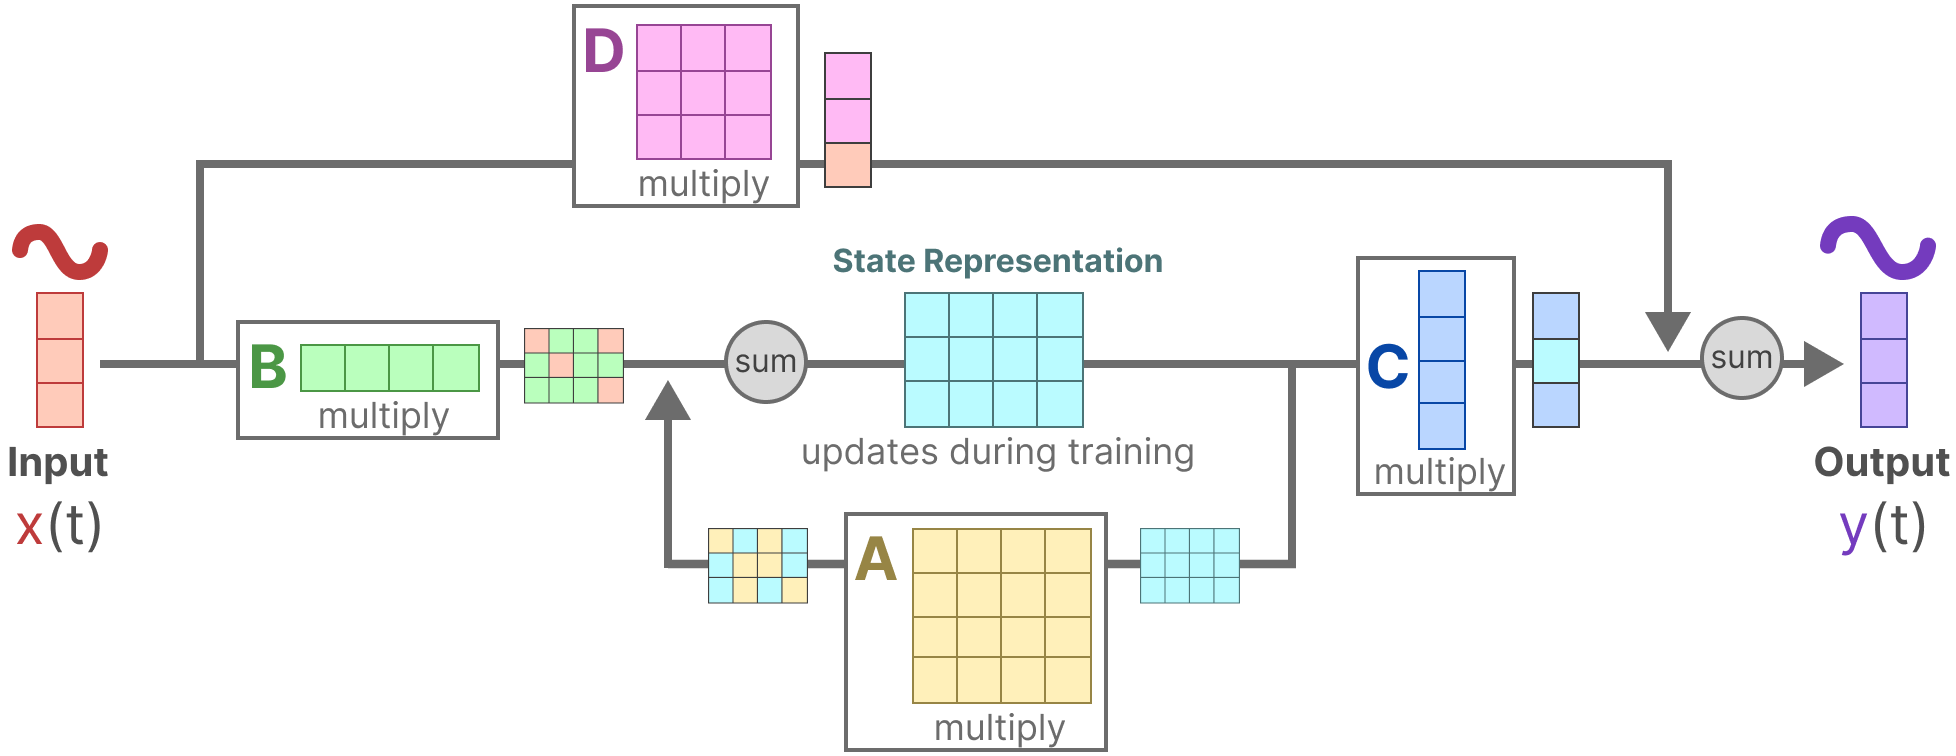
\includegraphics[width=0.9\linewidth]{./img/SSM_scheme.png}
    \end{center}
    \caption{Schemat modelu przestrzeni stanów.}\label{fig:ssm_scheme}
\end{figure}

\textcolor{blue}{Macierz $D$ przypomina połączenia rezydualne lub połączenia typu \textit{skip-connection} w głebokich sieciach neuronowych, które zapewniają inną ścieżkę dla danych, aby dotrzeć do ostatnich części sieci neuronowej poprzez pominięcie niektórych warstw \cite{resnet}. Dla uproszczenia zapisu często pomija się je w zapisie modelu}.

\subsubsection*{Dyskretyzacja modelu}
Modele tego typu działaja domyślnie w domenie danych ciągłych. Tekst lub muzyka są przykładami danych dyskretnych, przez co model musi zostać do nich dostosowany. Aby dokonać dyskretyzacji modelu wykorzystuje się metodę eksploratora (lub interpolatora) rzędu zerowego (\textit{ang. zero-order hold}). Metoda ta polega na podtrzymywaniu każdego otrzymanego sygnału, dopóki nie zostanie zapisany kolejny. Czas trwania poprzedniego sygnału jest dodatkowym parametrem nazywanym krokiem. W związku z tym, że model na wyjściu zwraca sygnał ciągły, aby zamienić go na dyskretny, należy próbkować go z odpowiednią długością kroku. Po dyskretyzacji modelu można nazwać go modelem \textit{sequence to sequence}. Aby lepiej zobrazować dokonane zmiany należy spojrzeć na równania \ref*{equ:rownanie_stanu_seq} oraz \ref*{equ:rownanie_wynikowe_seq}.


\begin{align}
     & \text{równanie stanu: }h_k = Ah_{k-1} + Bx_k \label{equ:rownanie_stanu_seq} \\
    \begin{split}
        &\text{równanie wynikowe: }y_k = Ch_k \label{equ:rownanie_wynikowe_seq} \\
    \end{split}
\end{align}

Model operuje teraz na sekwencjach a nie na sygnałach. Notacja została zmieniona z $t$ na $k$ aby lepiej zobrazować, że obecnie model pracuje na dyskretnych znacznikach czasu. Dodatkowo w zapisie równania usunięto macierz $D$.

\subsubsection*{Reprezentacja konwolucyjna}
Patrząc na zapis obu równań od razu można zaobserwować ich podobieństwo do rekurencyjnych sieci neuronowych. Każdy stan ukryty $h$ zależy w głównej mierze od stanu z \textcolor{blue}{poprzedniego} kroku czasowego. \textcolor{blue}{Modele przestrzeni stanów} mogą również być reprezentowane w postaci konwolucji. W związku z tym, że tekst lub muzyka są sekwencjami jednowymiarowymi w przeciwieństwie do typowego zastosowania sieci konwolucyjnych czyli obrazów, które są \textcolor{blue}{dwu- lub trzywymiarowe} należy zastosować \textcolor{blue}{jądro o wymiarze jeden.  Jednowymiarowa konwolucja działa poprzez przesuwanie filtru o ustalonej szerokości wzdłuż jednowymiarowego sygnału wejściowego, obliczając iloczyn skalarny wartości filtru i fragmentów sygnału w każdej pozycji. Wynik tej operacji tworzy nowy sygnał wyjściowy, który zawiera informacje o lokalnych cechach oryginalnego sygnału. W tym przypadku jądrem konwolucji (funkcji splotu) są odpowiednio przemnożone macierze $A, B$ oraz $C$, które są aktualizowane podczas treningu.} Tego rodzaju interpretacja modelu jest o tyle wygodna, że pozwala zrównoleglić trening modelu a co za tym idzie zmniejszyć jego czas \cite{ssm_notacja}. Kiedy model jest już wytrenowany i gotowy do generowania, można bez problemu przejść na interpretację rekurencyjną.

\subsubsection*{Macierz HiPPO}
Macierz $A$ modelu jest jego jednym z najistotniejszych elementów. To od niej zależy, czy model zapamięta cały kontekst wypowiedzi czy tylko kilka ostatnich tokenów. Jest to szczególnie ważne w przypadku predykcji, ponieważ model \textcolor{blue}{wykorzystuje jedynie ostatni stan ukryty}. Aby zapewnić dobrą kompresję kontekstu, jako $A$ stosuje się macierz HiPPO \cite{hippo}. Zadaniem macierzy \textit{\textbf{Hi}gh-order \textbf{P}olynomial \textbf{P}rojection \textbf{O}perators} jest jak najlepsze skompresowanie wejścia do wektora cech. Konstrukcję macierzy pokazano w równaniu \ref*{equ:hippo_matrix}. W tym przypadku można założyć, że macierz jest kwadratowa.

\begin{equation}
    A_{nk} = -
    \begin{cases}
        (2n + 1)^{1/2} (2k + 1)^{1/2} & \text{dla } n > k \\
        n + 1                         & \text{dla } n = k \\
        0                             & \text{dla } n < k
    \end{cases}
    \label{equ:hippo_matrix}
\end{equation}

Zbudowanie macierzy w taki sposób prowadzi do zdecydowanie lepszych wyników niż zainicjalizowanie jej losowo. Macierz HiPPO reprodukuje sekwencje w taki sposób, że dane, które są bliżej końca sekwencji są reprodukowane lepiej, niż te na początku. Ideą stojącą za używaniem takiego rozwiązania tp chęć zachowania jak największej liczby informacji w stanie ukrytym.

\subsubsection*{Modele 4S}
Po dodaniu omawianych usprawnień do tradycyjnego modelu SSM (dyskretyzacja, macierz HiPPO) nowo powstały model otrzymał nazwę \textit{Structured State Space for Sequences} (4S). Tego rodzaju modele pozwalają na śledzenie długich zależności w sekwencji dzięki macierzy HiPPO, a możliwość ich reprezentacji w postaci rekurencyjnej i konwolucyjnej rozwiązuje problemy między innymi złożoności obliczeniowej treningu oraz \textcolor{blue}{wykorzystywania modelu podczas prekcykcji.}

\subsection{Mamba}
Model Mamba posiada architekturę, która bazuje na modelach 4S, jednak wprowadza następujące usprawnienia.
\begin{enumerate}
    \item Algorytm selektywnego skanowania (\textit{selective scan}) pozwala skutecznie skupiać się na istotnych danych wejściowych i ignorować te nieistotne. Zdolność ta umożliwia lepszą obsługę zależności dalekiego zasięgu i filtrowanie szumów, co stanowi znaczną poprawę w stosunku do standardowych transformatorów, które traktują wszystkie dane wejściowe jako tak samo ważne.
    \item Algorytm \textit{hardware-aware}, który pozwala uniknąć konieczności wykonywania rozległych operacji wejścia/wyjścia pomiędzy różnymi poziomami hierarchii pamięci GPU, co prowadzi do znacznej poprawy szybkości operowania modelu.
\end{enumerate}

\begin{figure}[ht!]
    \begin{center}
        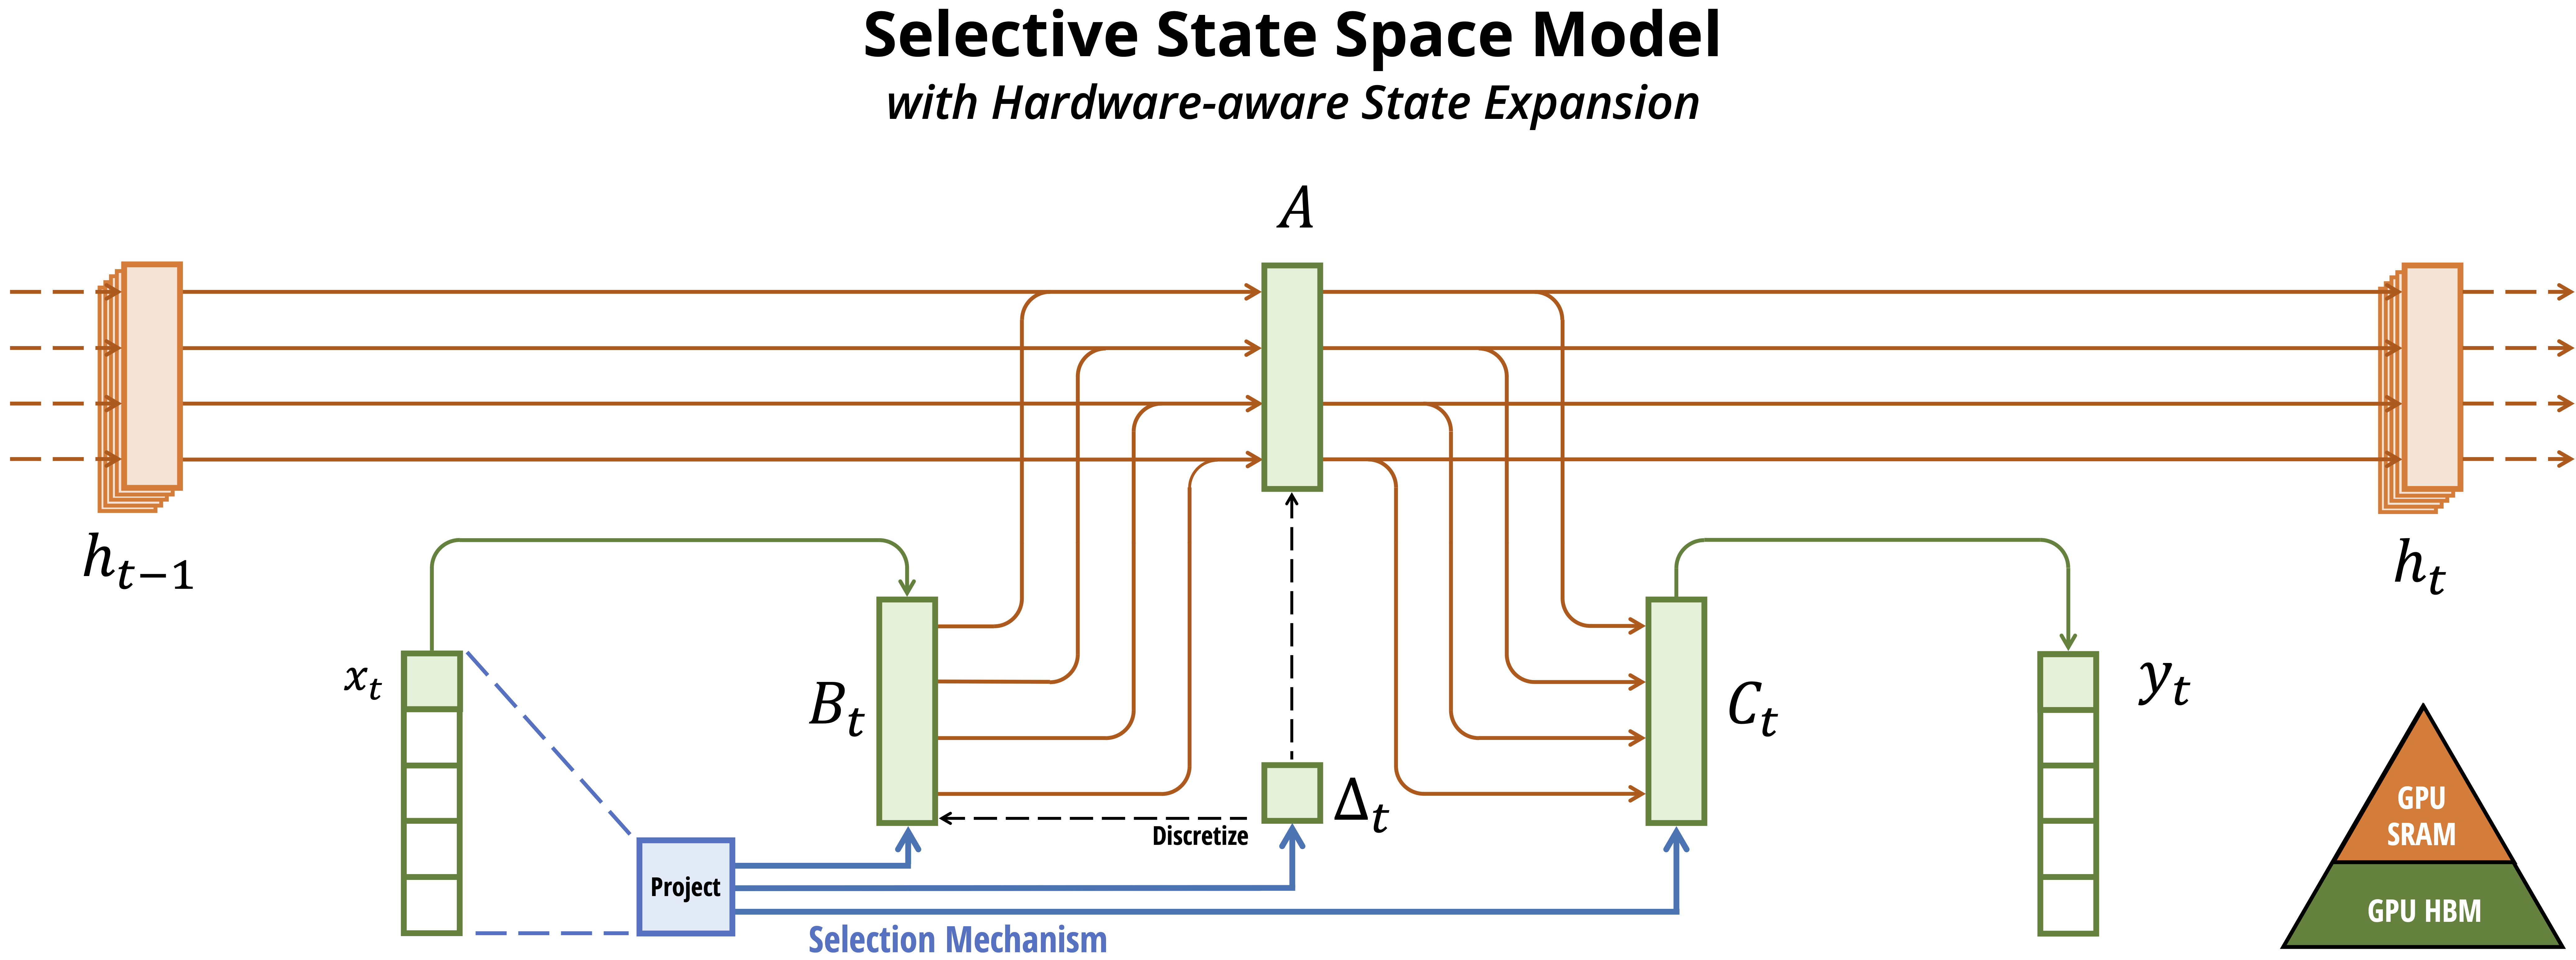
\includegraphics[width=0.9\linewidth]{img/mamba1.png}
    \end{center}
    \caption{Schemat modelu Mamba.}
    \label{fig:mamba1}
\end{figure}

Porównując grafiki \ref*{fig:mamba1} oraz \ref*{fig:ssm_scheme} można zobaczyć wiele podobieństw. Główne elementy pojawiają się w obu modelach, jednak w przypadku Mamby jest jasno zaznaczony jest mechanizm selekcji oraz dyskretyzacja modelu oznaczona jako $\Delta_t$. Model Mamba jest zoptymalizowany pod kątem specyficznych możliwości kart graficznych (GPU), na których jest on typowo uruchamiany i trenowany. Sekcje pamięci, na których są zaalokowane konkretne części modelu, na grafice są zaznaczone kolorem pomarańczowym i zielonym.

W przypadku zadań syntetycznych, takich jak kopiowanie sekwencji, Mamba nie tylko z łatwością rozwiązuje te zadania, ale może również ekstrapolować to rozwiązanie na bardzo długie sekwencje (ponad milion tokenów), których długość znacząco przewyższa tę, na której model został wytrenowany. Mamba osiąga wydajność jakości transformera w zadaniach modelowania języka zapewniając pięciokrotnie krótszy czas generowania w porównaniu do modeli transformerowych o podobnej wielkości i dorównuje wydajnością transformatorom dwukrotnie większym w testach porównawczych \cite{mamba}.

\chapter{Przeprowadzenie eksperymentów}
W celu oceny skuteczności modeli generowania muzyki, przeprowadzono szereg eksperymentów, w których porównano modele transformerowe oraz Mamba. Eksperymenty te były przeprowadzone na plikach muzycznych w formatach MIDI i ABC, a modele były trenowane w dwóch wariantach wielkościowych: z około 60 milionami parametrów oraz z 6 milionami parametrów. Celem tych badań było zrozumienie, jak różne podejścia i rozmiary modeli wpływają na jakość generowanej muzyki.

\section{Przygotowanie danych}
Pliki w formacie ABC, dzięki swojej tekstowej naturze, nie wymagały skomplikowanego przetwarzania wstępnego. Format ABC zapisuje nuty i inne informacje muzyczne w postaci tekstu, co idealnie pasuje do modeli przystosowanych do pracy z sekwencjami tekstowymi.

Do tokenizacji plików MIDI zastosowano algorytm REMI o którym była mowa w rozdziale \ref*{sec:REMI}. Przekształca on dane muzyczne w sekwencje tokenów, które mogą być interpretowane przez modele.

Aby jeszcze bardziej zredukować złożoność i objętość danych, zastosowano technikę \textit{Byte Pair Encoding} (BPE). BPE jest algorytmem kompresji tekstu, który jest szeroko stosowany w przetwarzaniu języka naturalnego do redukcji liczby unikalnych tokenów w sekwencjach tekstowych \cite{bpe}. W kontekście przetwarzania muzyki, BPE pomaga w optymalizacji danych wejściowych, co z kolei prowadzi do skrócenia sekwencji wejściowej modelu co przekłada sę na lepszej jakości predykcje \cite*{fradet2023byte}.

\noindent Algorytm można opisać w następujących krokach:

\begin{enumerate}
    \item Inicializacja: Każdy unikalny token (w kontekście muzyki będzie to nuta, pauza, zmiana tempa itp.) jest traktowany jako pojedynczy symbol.
    \item Zliczanie par: Algorytm identyfikuje najczęściej występujące pary sąsiadujących tokenów w sekwencji.
    \item Łączenie par: Najczęściej występujące pary są łączone w jeden nowy symbol, redukując tym samym liczbę symboli w sekwencji.
    \item Powtarzanie procesu: Kroki 2 i 3 są powtarzane, aż do osiągnięcia zdefiniowanego rozmiaru słownika \textit{(vocab size)}.
\end{enumerate}

\noindent Aby zilustrować działanie algorytmu BPE, można rozważyć prostą sekwencję liter \texttt{abcabcab}, na której zostanie przeprowadzony ten algorytm. Na początku należy zliczyć ilość par oraz zidentyfikować te najczęściej powtarzające się. W tym przypadku jest to para \texttt{ab}. Zostanie ona zamienione na nowy token np. \texttt{X}. Nowa sekwencja \texttt{XcXcX} zostaje poddana ponownej analizie z czego w tym przypadku wynika, że najczęstszą parą jest \texttt{Xc}. Zostanie ona zamieniona na nowy token \texttt{Y} z czego powstanie sekwencja \texttt{YYX}. W przypadku tekstu, tokenami na podstawie których obliczane są pary są kolejne bajty tekstu. W kontekście ztokenizowanego zbioru danych MIDI pary będą obliczane na podstawie tokenów takich jak: \texttt{Pitch\_C3}, \texttt{Velocity\_70}, \texttt{Duration\_1.0}. Jeśli tego rodzaju sekwencja będzie występowała wystarczająco często, to przy użyciu BPE zostanie ona zastąpiona jednym tokenem.

W przeprowadzonych eksperymentach ustawiono rozmiar słownika na 20,000, co zapewniło odpowiednią równowagę między kompresją a zachowaniem istotnych informacji muzycznych.

\section{Trening modeli}
HuggingFace to wiodąca firma w dziedzinie przetwarzania języka naturalnego i uczenia maszynowego, znana z opracowywania narzędzi i bibliotek ułatwiających tworzenie, wdrażanie i udostępnianie modeli uczenia maszynowego. Jednym z jej flagowych produktów jest bardzo popularna biblioteka typu \textit{open-source} Transformers, która zapewnia łatwy dostęp do szerokiej gamy wstępnie wytrenowanych modeli dla różnych zadań NLP, takich jak klasyfikacja tekstu, tłumaczenie, podsumowywanie i odpowiadanie na pytania. Biblioteka obsługuje modele takie jak BERT, GPT, T5 i wiele innych, oferując zarówno podstawową architekturę, jak i wstępnie wytrenowane wagi, co znacznie skraca czas i zasoby obliczeniowe potrzebne do dostrajania modeli. HuggingFace udostępnia wysokopoziomowe API pozwalające na tworzenie oraz trening modeli przy pomocy klas takich jak \texttt{Trainer}, \texttt{AutoModelForCausalLM} czy \texttt{ModelConfig}.

Jako reprezentant modelu transformerowego został wybrany model GPT-2 \cite{gpt2}. Model został stworzony przez OpenAI i jest to obecnie ich największy model udostepniony jako \textit{open source}. Jest oparty o architekturę \textit{decoder-only}.

Celem trenigu modeli typu \textit{Causal Language Model (CausalLM)} jest jak najwierniejsze przewidzenie następnego tokena w sekwencji, biorąc pod uwagę poprzednie tokeny. Podczas szkolenia tokeny wejściowe są wprowadzane do modelu, a model przewiduje rozkład prawdopodobieństwa nad wektorem tokenów, a nasępnie z takim prawdopodobieństwem losowany jest kolenjy token. Funkcja straty (\textit{loss}) jest obliczana na podstawie przewidywań modelu i rzeczywistych tokenów docelowych, które są tokenami wejściowymi przesuniętymi o jedną pozycję. Typowo używaną funkcją w tego rodzaju problemach jest funkcja entropii krzyżowej \textit{cross-entropy loss}, która mierzy różnicę między dwoma rozkładami prawdopodobieństwa: prawdziwym rozkładem (rozkładem docelowym) a rozkładem przewidywanym przez model.

W poniższych tabelach zostały pokazane konfiguracje modeli jak i liczba parametrów trenowanych modeli:

\begin{table}[!htb]
    % \begin{minipage}{.5\linewidth}
    \caption{Parametry modelu GPT-2}
    \centering
    \begin{tabular}{||c c c||}
        \hline
        Parametr          & model 6M & model 60M \\ [0.5ex]
        \hline\hline
        \texttt{n\_embed} & 128      & 512       \\
        \hline
        \texttt{n\_layer} & 2        & 6         \\
        \hline
        \texttt{n\_head}  & 1        & 4         \\
        \hline
        \texttt{n\_inner} & 256      & 2048      \\
        \hline
    \end{tabular}
\end{table}

\begin{table}[!htb]
    % \begin{minipage}{.49\linewidth}
    \caption{Parametry modelu Mamba}
    \centering
    \begin{tabular}{||c c c||}
        \hline
        Parametr                     & model 6M & model 60M \\ [0.5ex]
        \hline\hline
        \texttt{hidden\_size}        & 128      & 512       \\
        \hline
        \texttt{state\_size}         & 4        & 8         \\
        \hline
        \texttt{num\_hidden\_layers} & 8        & 12        \\
        \hline
    \end{tabular}
\end{table}

Parametry modelu GPT-2:
\begin{itemize}
    \item \texttt{n\_embed} - wymiarowość osadzeń oraz stanów ukrytych
    \item \texttt{n\_layer} - liczba warstw ukrytych w transformerze
    \item \texttt{n\_head} - liczba ,,głów'' w warstwach \textit{multi-headed attention} trasformera
    \item \texttt{n\_inner} - wymiar środkowych warstw typu \textit{feed-foreward}
\end{itemize}

Parametry modeli Mamba:
\begin{itemize}
    \item \texttt{hidden\_size} - wymiarowość osadzeń oraz stanów ukrytych
    \item \texttt{state\_size} -  rozmair stanów w modelu przestrzeni stanów
    \item \texttt{num\_hidden\_layers} - ilość warstw ukrytych modelu
\end{itemize}

\textcolor{blue}{Pomimo tego że istnieją pretrenowane modele generujące muzykę, w pracy został podjęty trening tego rodzaju modeli od samego początku. W związku z tym, że model Mamba jest dość nowym sposobem generowania sekwencji, nie powstały jeszcze modele muzyczne w tej architekturze, przez co porówywanie ich z pretrenowanymi modelami transformerowymi nie byłoby wiarygodnym testem.}

Trening modeli odbywał się na karcie graficznej NVIDIA Tesla A100. Czas trenigu modeli przedstawia wykres \ref*{fig:czas_treningu}. Każdy model były trenowany przez około 800 tysiecy kroków, jednak ich dokładna liczba różniła się pomiędzy eksperymentami. Aby lepiej przedstawić różnice w czasie trenigu na wykresie przedstawiono tylko czas pierwszych 100 tysiecy kroków. Modele trenowane na plikach ABC, wymagały zdecydowanie krótszego czasu trenigu, co wynikało z mniejszej ilości unikatowych tokenów w stosunku do reprezentacji MIDI.

\begin{figure}[ht!]
    \centering
    \begin{tikzpicture}
        \begin{axis}[
                width = 14cm,
                height = 8cm,
                ybar,
                symbolic x coords={Mamba 6M, Mamba 60M, GPT2 6M, GPT2 60M},
                xtick=data,
                nodes near coords,
                ymin=0,
                % xlabel={Modele},
                ylabel={Czas treningu w $h$},
                bar width=15pt,
                enlarge x limits=0.3,
                enlarge y limits={value=0.2, upper}
            ]
            \addplot coordinates {(Mamba 6M, 2.924) (Mamba 60M, 3.748) (GPT2 6M, 1.774) (GPT2 60M, 8.218) };
        \end{axis}
    \end{tikzpicture}
    \caption{Czas trenigu 100 tysięcy kroków modeli.}\label{fig:czas_treningu}
\end{figure}

Porównując czasy treningu obu architektur można dojść do następujących wniosków. Dość oczywistą obserwacją jest fakt, że trening modeli mniejszych jest krótszy niż tych większych. Pomimo tego, że model Mamba powinien trenować się szybciej niż modele transformerowe, nie jest to prawdą dla mniejszego modelu. Model transformerowy GPT2 6M trenował się o 39.4\% szybciej niż jego odpowiednik w konkurencyjnej architekturze. Różnica w szybkości treningu jest zdecydowanie bardziej widoczna w dużych modelach, gdzie model transformerowy GPT2 60M trenował się prawie 120\% dłużej niż model Mamba o tej samej liczbie parametrów. Na podstawie tych obserwacji można stwierdzić, że w kontekście dużych modeli, architektura Mamba jest bardziej efektywna pod względem czasu treningu niż architektura GPT2.

\begin{figure}[ht!]
    \centering
    % \begin{tikzpicture}
    %     \begin{axis}[
    %             width=14cm,
    %             height=8cm,
    %             % xmin=0, xmax=1e4,
    %             % ymin=1e-4, ymax=1e-1,
    %             scaled x ticks=false,
    %             xlabel={Liczba kroków},
    %             ylabel={Wartość \textit{loss}},
    %             % label style={font=\bfseries\boldmath},
    %             % tick label style={font=\bfseries\boldmath},
    %         ]
    %         \addplot[scatter, no marks, draw=blue!60]
    %         table [x=index, y=Mamba_60M, col sep=comma] {data.csv};
    %         \addplot[scatter, no marks, draw=red!60]
    %         table [x=index, y=Mamba_6M, col sep=comma] {data.csv};
    %         \addplot[scatter, no marks, draw=orange!60]
    %         table [x=index, y=GPT2_60M, col sep=comma] {data.csv};
    %         \addplot[scatter, no marks, draw=green!60]
    %         table [x=index, y=GPT2_6M, col sep=comma] {data.csv};
    %     \end{axis}
    % \end{tikzpicture}
    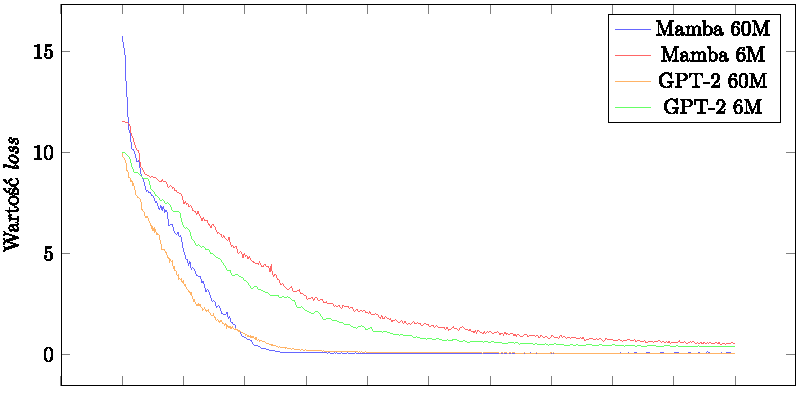
\includegraphics[width=0.9\linewidth]{./img/training_plot.pdf}
    \caption{Wykresy treningu pierwszych 250 tysięcy kroków modeli.}\label{fig:midi_train}
\end{figure}

Na grafice \ref*{fig:midi_train} przedstawiono wartość funkcji straty podczas trenigu modeli. W celu dokonania lepszej wizualizacji ograniczono ilość kroków do 250 tysięcy. Modele z większą liczbą parametrów (60M) szybciej osiągnęły niższą funkcję straty w porównaniu do modeli z mniejszą liczbą parametrów (6M). Dzieje się tak, ponieważ większe modele mają lepszą zdolność do reprezentowania skomplikowanych zależności w danych przy pomocy swoich parametrów dzięki czemu mogą lepiej dopasować się do zbioru treningowego, co prowadzi do szybszej redukcji funkcji straty. Pomimo tego, że duże modele osiągnęły niższe wartości szybciej, wszystkie modele wytrenowały się do podobnego poziomu.

\begin{figure}
    \centering
    \begin{tikzpicture}
        \begin{axis}[
                width=14cm,
                height=8cm,
                xlabel={Liczba tokenów},
                ylabel={Czas generowania [$s$]},
                xtick=data,
                xticklabels from table={data.dat}{date},
                legend pos= north west
            ]
            \addplot[color=blue!60, mark=*] table[x expr=\coordindex, y=Mamba_60M] {data.dat};
            \addplot[color=red!60, mark=square*] table[x expr=\coordindex, y=Mamba_6M] {data.dat};
            \addplot[color=orange!60, mark=triangle*] table[x expr=\coordindex, y=GPT2_60M] {data.dat};
            \addplot[color=green!60, mark=diamond*] table[x expr=\coordindex, y=GPT2_6M] {data.dat};
            \legend{Mamba 60M, Mamba 6M, GPT2 60M, GPT2 6M}
        \end{axis}
    \end{tikzpicture}
    \caption{Czas generowania tokenów przez modele.}\label{fig:time_generate}
\end{figure}

Na grafice \ref*{fig:time_generate} przedstawiono czas generowania konkretnej liczby tokenów przez modele. Najszybciej działa najmniejszy model GPT2, gdzie dla każdej wartości generuje sekwencje poniżej jednej sekundy. Porównując duże modele, widać że Mamba radzi sobie lepiej, szczególnie dla dłuższych sekwenji, działając prawie dwa razy szybciej. Dużym zasokoczeniem jest gwałtowny wzrost czasu dla modelu Mamba 6M.

\textcolor{blue}{Przyglądając się małemu oraz dużemu modelowi Mamby, można zauważyć, }że różnica między nimi nie jest tak duża jak w przypadku modeli GPT2. Może wynikać to z tego, że model ten w swojej architekturze jest zoptymalizowany pod kątem obsługi bardzo dużej liczby parametrów. Najmniejszy model jaki został wytrenowany i udostępniony przez twórców tej architektury posiadał 128 milionów parametrów, co może sugerować, że dużo mniejsze modele nie zachowują obiecywanych zalet związanych z ich osiągami.

\section{Prezentacja otrzymanych wyników}
Przedstawienie muzyki w pracy stanowi wyzwanie w porównaniu na przykład do wizualnych form sztuki, takich jak obrazy. Muzyka jest medium audytywnym, które oddziałuje na słuch i emocje poprzez dźwięki i rytm, co sprawia, że jej pełne doświadczenie jest trudne do przekazania za pomocą samego tekstu. Opisy muzyczne, notacja i partytury mogą dostarczyć informacji o strukturze i elementach utworu, ale nie oddają one w pełni jego brzmienia i atmosfery. W przeciwieństwie do obrazów, które można bezpośrednio zobaczyć i ocenić na papierze, muzyka wymaga aktywnego odtwarzania, by w pełni ją zrozumieć i docenić. W pracy zostaną przedstawione generacje w dwojaki sposób. W zależności od tego, czy model był wytrenowany na plikach MIDI lub notacji ABC, będzie przedstawiony wynik modelu w formie tekstowej lub \textit{piano roll}. Dodatkowo do każdego z tych przykładów zostanie dodana wygenerowana partytura, jednak należy pamiętać, że w związku z tym, że pliki MIDI są zapisem odegrania muzyki a nie samej jej notacji, reprezentacja plików MIDI na pięciolinii potrafi nie być idealna co jest spowodowane możliwymi nieregularnościami w rytmie.

Na grafice \ref*{code:music_gen1} przedstawiono wynik modelu GPT-2 60M w wersji ABC. Część oznaczoną kolorem niebieskim należy traktować jako sekwencje wejściową dla modelu, na której podstawie model generuje kolejne tokeny. Dodatkowo zostały podane kody kontrolne \texttt{S}, \texttt{B} oraz \texttt{E}. Reprezentacje otrzymanej muzyki zapisanej na pięciolinii przedstawia grafika \ref*{fig:music_gen1}.

Należy zwrócić uwagę, że model został poproszony o wygenerowanie melodii w tonacji C-dur (\texttt{K:C}), jednak jak można zaobserwować na obu reprezentacjach, model zignorował tą część zapytania i wygenerował melodię w tonacji d-moll. Prawdopodobnie wzięło się to z faktu, że podane jako początek sekwencji dźwięki \texttt{d}, nie są typowym rozpoczęciem melodii w tonacji C-dur. Model oczekiwał podania toniki (pierwszego stopnia skali) ponieważ takie fragmenty są najbardziej popularne i dominowały zbiór uczący. Kody kontrolne są dodawane do zbioru danych, jednak model nie jest bezpośrednio penalizowany podczas treningu za to, że ich się nie trzyma. Pomimo tego, większość melodii wygenerowanych przez modele trzymają się podanych kodów. W tabeli [tautaj ref będzie] zostało przedstawione porównanie dwudziestu wygenerowanych 
\begin{comment}
Tutaj jutro dodam tabelkę z tym 
\end{comment}

\begin{figure}
    \begin{minted}[breaklines,escapeinside=++,breaksymbolleft=,linenos=false]{text}
+\textcolor{blue}{X:1}+
+\textcolor{blue}{S:2}+
+\textcolor{blue}{B:9}+
+\textcolor{blue}{E:4}+
+\textcolor{blue}{L:1/8}+
+\textcolor{blue}{M:3/4}+
+\textcolor{blue}{K:C}+
+\textcolor{blue}{D/2d/2d}+ Ad fa | a/g/e/f/ g/f/e/d/ ^cA | d2 dA df | ag/f/ e^c A2 | D2 d^c de | f2 ef/g/ a/g/f/e/ | d2 df e^c |1 d2 D4 :| 2 d2 D2 fg |: a2 g2 f2 | ed ^cd e/f/g | a2 g2 f2 | ed ^cd e/f g | a2 g2 f2 | ed ^cd ef/g/ | a2 g2 fe |1 d2 de fg :|2 d2 D4 ||
    \end{minted}
    \caption{Wynik modelu.}\label{code:music_gen1}
\end{figure}


\begin{figure}[ht!]
    \begin{center}
        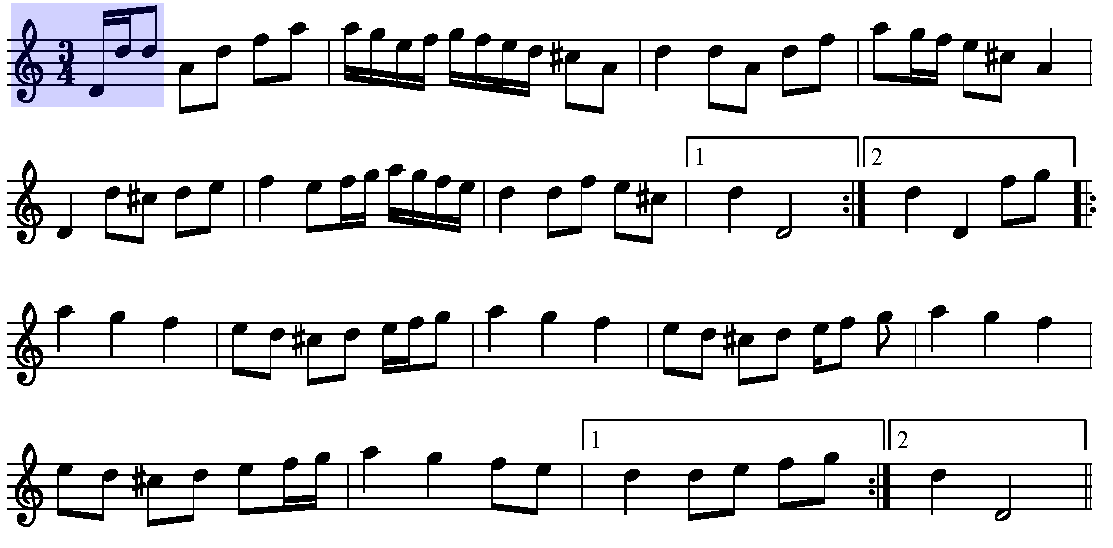
\includegraphics[width=0.9\linewidth]{./img/abc_gen_nice1.pdf}
    \end{center}
    \caption{Wygenerowana melodia ABC.}\label{fig:music_gen1}
\end{figure}

Generowanie plików MIDI jest bardziej skomplikowanym procesem w przeciwieństwie to tego z plików ABC, gdzie wystarczy przy pomocy klawiatury wprowadzić odpowiednie nuty. W tym przypadku, predykcje są powiązane z tokenizatorem, który zamienia konkretne dźwięki na tokeny, które są rozumiane przez model. Najprostrzym sposobem, jest stworznie początku sekwencji przy pomocy dowolnego edytora plików MIDI, a następnie otwarcie ich przy pomocy odpowiedniej bilbioteki oraz zamianę na tokeny przy pomocy tego samego tokenizatora, który został użyty podczas treningu modelu.

Przykładowe predykcje stworzone przy pomocy modelu Mamba 6M można zobaczyć na grafikach \ref*{fig:music_genMIDI_notes} oraz \ref*{fig:music_genMIDI}.

\begin{figure}[ht!]
    \begin{center}
        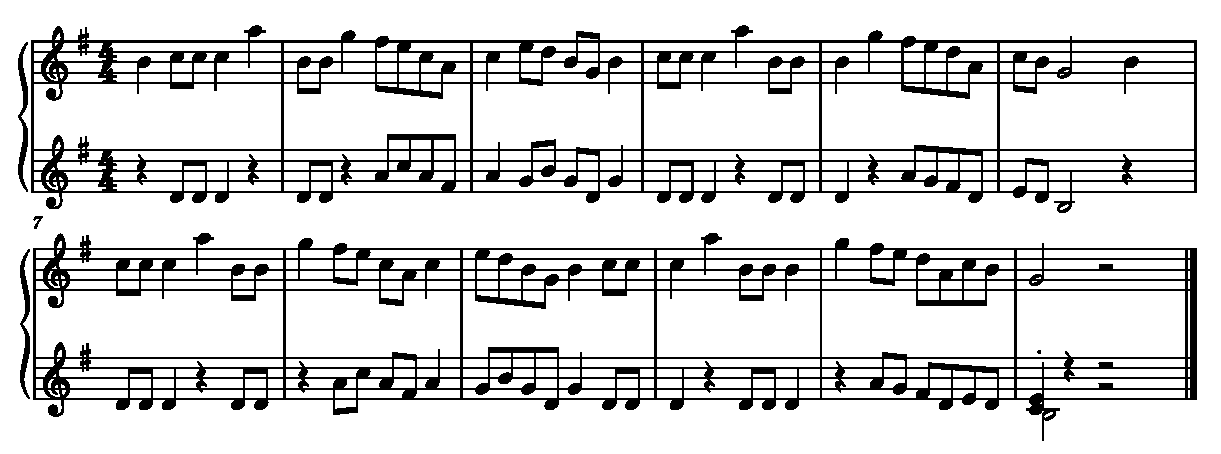
\includegraphics[width=0.9\linewidth]{./img/35.pdf}
    \end{center}
    \caption{Wygenerowana melodia MIDI zapisana w notacji muzycznej.}\label{fig:music_genMIDI_notes}
\end{figure}

\begin{figure}[ht!]
    \begin{center}
        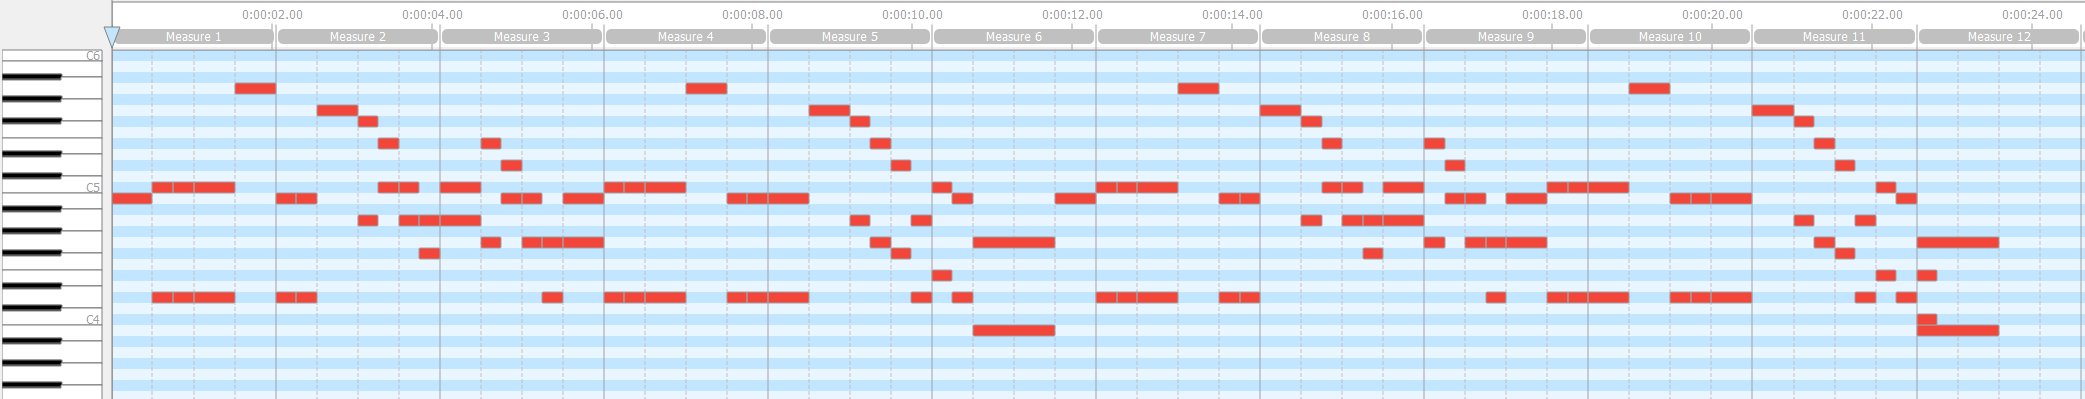
\includegraphics[width=0.9\linewidth]{./img/midi_generated.png}
    \end{center}
    \caption{Wygenerowana melodia MIDI.}\label{fig:music_genMIDI}
\end{figure}

Różnicą, która jest widocza pomiędzy precykcjami \ref*{fig:music_genMIDI_notes} oraz \ref*{fig:music_gen1} jest sposób generowania powtórzeń w muzyce. W notacji ABC odbywa się to przy pomocy znaków notacji muzycznej, które mówią o tym jakie fragmenty mają zostać powtórzone. W przypadku predykcji plików MIDI, w drugiej linijce wygenerowanego fragmentu występuje powtórzenie pierwszej linijki (poza ostatnim taktem), które mogłby zostać zapisane na pięciolini przy pomocy odpowiednich znaków. Modelowi udało się zapamiętać i poprawnie odtworzyć wcześniej wygenerowaną sekwencję, co nie zawsze może się wydarzyć.

W pracy zostały przedstawione fragmenty, które zostały wybrane przez autora jako wyjątkowo dobre i brzmiące wiarygodnie, jednak nie wszystkie predykcje należą do tej grupy. Część predykcji jest nieudanymi próbami modelu, do generowania muzyki, która zwyczajnie nie brzmi dobrze. Część fragmentów kończy się za szybko, ponieważ model dodał w nich znak końca sekwencji w niepoprawnym miejscu lub fragmenty zawierają zdecydowanie zbyt dużą liczbę pauz następujących po sobie, co wprowadza dość niezręczną ciszę w wygenerowanych fragmentach. Zdecydowanie większa część udanych generacji modelu powstała na podstawie plików ABC, co jest następstwem prostrzej stuktury tych plików. Również w przypadku tego formatu, co jest szczególnie widoczenie kiedy model jest niedotrenowany, model jest w stanie wygenerować sekwencje, które nie są zgodne z notacją, przez co nie są one możliwe do odsłuchania w dostępnym oprogramowaniu. Takie fragmenty, należy pomijać, lub próbować poprawiać je ręcznie.

\section{Sposoby oceny wyników}
Celem porównania otrzymanych wyników z dowolnych modeli, jest ocena jakości ich pracy. W kontekście modeli dyskryminujących (ang. \textit{discriminative model}), na przykład klasyfikatorów bądź modeli regresyjnych, ocena ich jakości jest dość prosta, ponieważ istnieje predefiniowana, prawdziwa wartość w zbiorze testowym, którą model próbuje przewidzieć. W takim przypadku ewaluacja jakości modelu to porównanie prawdziwych danych, z tymi przewidzianymi przez model. Porównanie odbywa się przez policzenie metryk np. dla modelu klasyfikującego celności, precyzji, \textit{F1-score} lub dla modelu regresyjnego MSE lub $R^2$. W przypadku modeli generatywnych celem treningu jest jak najlepsza aproksymacja rozkładu prawdopodobieństwa danych $P(X_{data})$ lub w przypadku danych oznaczonych łączny rozkład $P(X, Y)$. W przypadku dużej wymiarowości danych, obliczenie obiektywnych metryk takich jak \textit{log-likelihood} lub dywergencja Kullbacka-Leiblera (\textit{KLD}) często jest nieobliczalne. Dla człowieka weryfikacja wyników modeli generatywnych takich jak \textit{text-to-speech} lub \textit{text-to-image} jest trywialnym zadaniem, jednak nie jest to oczywiste zadanie algorytmiczne. Często odwołuje się do subiektywnych metryk takich jak (\textit{MOS ang. mean opinion score}), które oblicza się jako średnią opinię na przykład w skali od 1-5 braną z zazwyczaj niewielkiej grupy ludzi. Niestety metryka ta często nie jest wiarygodna ze względu na jej subiektywnośś oraz niewielką próbę badawczą. Aby wyeliminować te wady serwisy takie jak HuggingFace udostępniają narzędzia dla członków społeczności, które pozwalają na ranking modeli, z nadzieją że zgodnie z prawem wielkich liczb, przy wystarczającej liczbie odpowiedzi, uda się otrzymać w miarę obiektywną ocenę. Przykładowym narzędziem tego rodzaju jest \textit{The TTS Arena}\cite{tts_arena}, która pozwala na ranking modeli \textit{text-to-speech}.

W przypadku muzyki, istnieje możliwość aby zweryfikować poprawność wygenerowanych sekwencji odwołując się do teorii oraz harmonii muzyki. Istnieje kilka narzędzi takich jak \textit{Chordify}, \textit{Hooktheory} lub \textit{Sibelius}, które pozwalają na analizę harmoniczną utworów, dzieki czemu autorzy mogą w prosty sposób analizować i dobierać progresję danej melodii. Niestety większość takich narzędzi jest płatna i nie pozwala na zautomatyzowaną analizę wielu plików. Dodatkowym problemem jest w analizie harmonicznej, szczególnie prowadzonej przez algorytmy, jest rozróżnienie harmonii wertykalnej oraz horyzontalnej. Rozróżnienie to zostało wytłumaczone przez Jacoba Colliera, kilkukrotnego laureata nagród \textit{Grammy}, którego zdaniem akord, który nawet zagrany sam brzmi niepoprawnie, w odpowiednim kontekście i przez odpowiednią progresję w kolejnych fragmentach muzyki, może mieć nadany sens, przez co cała sekwencja nabiera muzycznego piękna \cite{collier_wrongnote}.

Brak obiektywnych metryk, którymi można się posłużyć podczas ewaluacji modelu jest dodatkowym problemem w momencie \textit{fine-tunigu} modelu. Ciężko jest wybrać odpowiednie rozwiązanie architektoniczne lub odpowiednie hiperparametry, kiedy jedyną miarą jakości wygenerowanych danych jest subiektywna opinia programisty lub grupy osób wybranych jako wyrocznia.

\subsection{Testowanie melodii innymi LLM-ami}
Aby zweryfikować jakość predykcji, można zastosować podejście polegające na wytrenowaniu innego modelu na danych muzycznych. Tym sposobem powstanie model, który będzie w stanie ocenić oraz udzielić konstruktywnej krytyki na temat przedstawionego mu fragmentu muzycznego.
\subsubsection*{ChatMusician}
\textit{ChatMusician} to otwarty model językowy, który integruje zdolności muzyczne \cite{yuan2024chatmusician}. Model ten został zaprojektowany na bazie modelu LLaMA2 z siedmioma miliardami parametrów, jest trenowany i dostrajany z wykorzystaniem notacji muzycznej ABC, traktując muzykę jako drugi język. Dzięki temu ChatMusician jest w stanie rozumieć i generować muzykę za pomocą tekstowego tokenizatora, bez konieczności stosowania zewnętrznych struktur neuronowych czy tokenizatorów stworzonych specjalnie dla notacji muzycznej. \textit{ChatMusician} może komponować dobrze zorganizowane, pełnometrażowe utwory muzyczne na podstawie tekstu, akordów, melodii, motywów i form muzycznych, przewyższając wyniki modelu GPT-4. Model ten osiąga lepsze wyniki niż LLaMA2 i GPT-3.5 w zadaniach związanych z rozumieniem teorii muzyki, co potwierdzono w benchmarku \textit{MusicTheoryBench}, zaprojektowanym do oceny zdolności modeli do rozumienia i rozumowania muzycznego. Model został udostepniony dla użytku publicznego na platformie HuggingFace.

Model jest potencjalnym rozwiązaniem problemu z oceną wygenerowanej muzyki. Będąc wytrenowanym na prawdziwych fragmentach muzycznych z całego świata i wielu kultur oraz tekstu zawierającego teorię muzyki, powinien w dość obiektywny sposób oceniać fragmenty melodii. Pytanie zadane do modelu brzmi następująco: ,,Wygenerowałem muzykę w notacji ABC. Czy mógłbyś ją przeanalizować i powiedzieć, czy brzmi naturalnie? W szczególności chciałbym prosić o opinię na temat ogólnej muzykalności, poczucia harmonii i tego, czy melodia i progresje akordów są spójne i przyjemne. Oto jej notacja:''. W związku z tym, że model działa tylko dla języka angielskiego należy przetłumaczyć pytanie na ten własnie język.

Zapytanie o wygenerowany fragment zapisany na partyturze \ref*{fig:music_gen1} przedstawiono na \ref*{code:chat_prompt1}.

\begin{figure}[ht!]
    \begin{minted}[breaklines,escapeinside=++,breaksymbolleft=,linenos=false]{text}
+\textcolor{red}{PROMPT:}+ I have some music in ABC notation that I generated. Could you analyze it and tell me if it sounds natural? Specifically, I would like your feedback on the overall musicality, the sense of harmony, and whether the melody and chord progressions are coherent and pleasing. Here is the ABC notation of the music:
X:1
L:1/8
M:3/4
K:C
D/2d/2d Ad fa | a/g/e/f/ g/f/e/d/ ^cA | d2 dA df | ag/f/ e^c A2 | 
D2 d^c de | f2 ef/g/ a/g/f/e/ | d2 df e^c |1 d2 D4 :|2 d2 D2 fg |:
a2 g2 f2 | ed ^cd e/f/g | a2 g2 f2 | ed ^cd e/f g | a2 g2 f2 | 
ed ^cd ef/g/ | a2 g2 fe |1 d2 de fg :|2 d2 D4 ||
    \end{minted}
    \caption{Pytanie dla modelu ChatMusician.}\label{code:chat_prompt1}
\end{figure}

\begin{figure}[ht!]
    \begin{minted}[breaklines, escapeinside=++,breaksymbolleft=,linenos=false]{text}
+\textcolor{red}{ANSWER:}+ Overall Musicality: 1. The piece has a pleasant and flowing rhythm with a steady tempo. It features a mix of different instruments andvoices, creating an interesting texture. The melodies are catchy and memorable, making the piece enjoyable to listen to. 2. Sense of Harmony: The harmonies in this piece are well-crafted and create a rich and full sound. The use of various chords and progressions adds depth and complexity to the music. The harmonic choices are appropriate for the style and genre of the piece. 3. Melody and Chord Progressions: The melody and chord progressions in this piece are coherent and pleasing. They follow a logical progression and fit together well. The melodic lines are well-written and expressive, adding to the emotional impact of the piece. The chord progressions provide a solid foundation for the melodies and add interest and variety to the composition.In conclusion, this piece of music has a strong sense of musicality, harmony, and coherence. The melodies and chord progressions are well-constructed and contribute to the overall appeal of the piece. It is a successful example of its genre and style.
    \end{minted}
    \caption{Odpowiedź modelu ChatMusician.}\label{code:chat_answer1}
\end{figure}

Model dość przychylnie spojrzał na ten wygenerowany fragment, jednak jego odpowiedzi nie są specyficzne o czym można się przekonać czytając odpowiedź na grafice \ref*{code:chat_answer1}. Nie podejmuje on analizy konkretach fragmentów i dodatkowo udziela informacji o użytych wielu instrumentach, co nie występuje w przedstawionym mu fragmencie. W kontekście harmonii używa słów takich jak \textit{well-crafted}, \textit{coherent}, \textit{pleasing}. Słowa te są bardzo ogólne i nie stanowią dobrej analizy fragmentu muzycznego. Dodatkowo w opinii udzielonej przez model występują powtorzenia, które dodatkowo zmniejszają wiarygodność oceny. Model nie udzielił żadnej negatywnej odpowiedzi lub nie zasugerował możliwości zmiany.

Aby upewnić się czy udzielania wyłącznie pozytywnych informacji nie jest domyślnym zachowaniem modelu należy poprosić model o ocenę fragmentu, który został specjalnie przygotowany, aby nie brzmiał dobrze dla ludzkiego ucha. Zapis tego fragmentu został zapisany na grafice \ref*{fig:gen_bad}. Dodatkowo, pomimo tego że zapis jest poprawny w notacji ABC, niektóre takty zawierają więcej lub mniej dźwięków niż jest to przewidziane w metrum \musFig{4 4}. Odpowiedź modelu przedstawiono we fragmencie \ref*{code:chat_prompt2}.

\begin{figure}[ht!]
    \begin{center}
        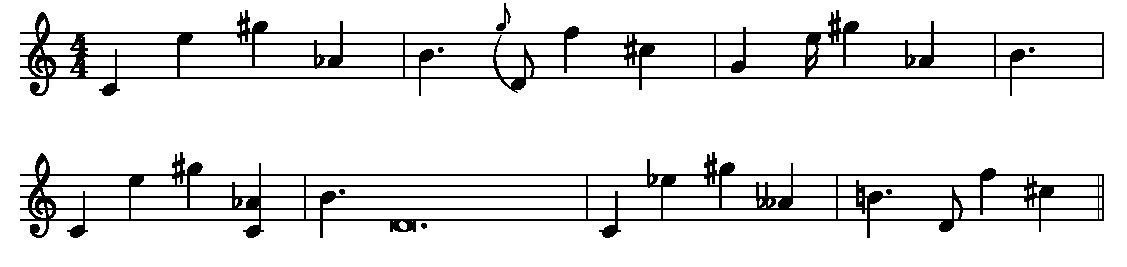
\includegraphics[width=0.9\linewidth]{./img/abc_gen_notnice1.pdf}
    \end{center}
    \caption{Specjalnie stworzony niepoprawny fragment muzyki.}\label{fig:gen_bad}
\end{figure}

\begin{figure}[ht!]
    \begin{minted}[breaklines,escapeinside=++,breaksymbolleft=,linenos=false]{text}
+\textcolor{red}{ANSWER:}+ Overall Musicality: The piece has a pleasant and flowing
quality to it, with a mix of different rhythms and tempos. The use of 
dynamics and articulations adds depth and interest to the composition. 
2. Sense of Harmony: The harmonies used in this piece are mostly consonant 
and create a sense of stability and balance. There are occasional 
dissonances that add tension and color to the music. 3. Melody and Chord 
Progressions: The melodies in this piece are well-crafted and follow a 
logical progression. They are easy to sing or play and have a clear 
sense of direction. The chord progressions are also coherent and support 
the melodies effectively. In conclusion, this piece has a good overall 
musicality, sense of harmony, and coherence between its melody and 
chord progressions. It is an enjoyable and engaging composition.
    \end{minted}
    \caption{Odpowiedź modelu na fałszywy fragment.}\label{code:chat_prompt2}
\end{figure}

Obie opinie są bardzo do siebie podobne. Okazuje się, że model nie jest w stanie dobrze rozpoznawać to, czy muzyka jest rzeczywiście przyjemna dla ucha czy nie. Nie wychwycił problemów z rytmem, które nie jest jednakowe dla każdego taktu oraz nie wyraził żadnej konstruktywnej krytyki. Niestety model \textit{ChatMusician} nie jest dobrym rozwiązania jeśli chodzi o ocenianie muzyki.

\subsubsection*{GPT-4}
% estimates 1.76 trillion parameters
Aby porównać możliwości oceny modeli LLM nalezy użyć silniejszego modelu. GPT-4 to model, który obecnie najlepiej wypada na praktycznie każdym benchmarku \cite{openai2024gpt4}. W porównaniu do swojego poprzednika, GPT-3, charakteryzuje się większą liczbą parametrów, co pozwala mu na lepsze rozumienie i generowanie skomplikowanych tekstów. GPT-4 potrafi również wykazywać większą spójność i koherencję w dłuższych wypowiedziach, lepiej interpretować kontekst oraz odpowiadać na bardziej złożone pytania. W związku z tym, że model nie jest \textit{open source} jego dokłada konfiguracja nie jest znana, jednak hipotetyzuje się, że ma 1.67 trylionów parametrów \cite{leakgpt4}. Nie był on trenowany bezpośrednio na danych muzycznych, jednak przez swój rozmiar, który jest potencjalnie aż o ponad 2000 razy większy od modelu \textit{ChatMusician}, powinien posiadać przynajmniej podstawową znajomość muzyczną. Wadą tego rozwiązania jest fakt, że GPT-4 jest dostępny jedynie po wykupieniu subskrypcji na stronie OpenAI, która kosztuje 20\$ na miesiąc.

Do modelu zostało przekazane takie samo pytanie jak w wyżej opisanym przypadku.
\begin{minted}[breaklines,fontsize=\tiny,breaksymbolleft=,linenos=false]{text}
To evaluate the musicality and harmony of your ABC notation, I will provide an analysis based on the key, melody, rhythm, and chord progressions. Here is a detailed breakdown of your piece:

### Key and Meter
- **Key:** C major
- **Meter:** 3/4 (Waltz time)

### Melody and Harmony
1. **Opening Phrase:**
   - `D/2d/2d Ad fa | a/g/e/f/ g/f/e/d/ ^cA`
     - This phrase introduces a mix of stepwise motion and leaps, giving a dynamic start. The alternation between the upper and lower notes creates a call-and-response effect. The use of the raised 4th degree (^c) adds a touch of chromaticism.

2. **Middle Phrase:**
   - `d2 dA df | ag/f/ e^c A2`
     - The repetition of 'd' with variations in intervals suggests a thematic consistency. The leap to 'f' and back to 'd' maintains interest. The movement towards 'A' anchors the phrase back to the tonic's dominant, providing harmonic stability.

3. **Transition:**
   - `D2 d^c de | f2 ef/g/ a/g/f/e/`
     - The use of the D minor chord (D-F-A) transitioning to E minor (E-G-B) and then back to fragments of D minor adds tension and resolution.

4. **Closing Phrase:**
   - `d2 df e^c |1 d2 D4 :|2 d2 D2 fg`
     - This phrase returns to the tonic D and introduces a cadential figure (D-F-E-^C). The first ending resolves to the tonic D major chord, while the second ending moves into a continuation with 'fg', creating a sense of forward motion.

### Second Part
1. **Opening Phrase:**
   - `a2 g2 f2 | ed ^cd e/f/g`
     - This section starts with a descending sequence, providing contrast to the first part. The melodic minor descent with a chromatic touch (e-^c-d) maintains interest.

2. **Middle Phrase:**
   - `a2 g2 f2 | ed ^cd e/f g`
     - The repetition reinforces the theme while subtle variations in articulation (slurs) add expressiveness.

3. **Transition and Closing:**
   - `a2 g2 f2 | ed ^cd ef/g/ | a2 g2 fe`
     - The alternation between stepwise motion and leaps ensures coherence and variety. The repeated 'a-g-f' figure creates familiarity, while 'e-^c-d ef/g/' keeps it fresh.

4. **Final Cadence:**
   - `1 d2 de fg :|2 d2 D4 ||`
     - The final cadence resolves nicely with the repeating 'de fg' figure leading to the tonic 'D' again, ensuring a satisfying conclusion.

### Overall Musicality
- **Melodic Coherence:** The melody has a clear direction with a good mix of stepwise motion and leaps, maintaining interest.
- **Harmony:** The harmony is mostly implied through the melodic line with occasional chromatic touches adding tension and resolution. The frequent returns to tonic and dominant notes (C and G) provide a sense of harmonic stability.
- **Rhythmic Flow:** The piece maintains a consistent waltz rhythm (3/4 time), which gives it a dance-like quality, adding to its musicality.

### Conclusion
The piece sounds natural and coherent, with a pleasing melody and harmonic progression. The use of chromatic notes and variations in articulation adds interest and depth. It effectively balances repetition with variation, ensuring both familiarity and novelty for the listener.
\end{minted}

Jak można zauważyć ocena fragmentu muzyki przez GPT-4 jest dość długa oraz bardzo dokładna. Podczas analizy rozbija muzyke na główne fragmenty, a następnie każdy z tych fragmentów poddaje szczegółowej analizie rozdzielając je dalej na początek, środek, przejście i zakończenie. Dla każdej z wyróżnionych części udziela konkretnej analizy harmonicznej, mówiącej o progresję akordów używając technicznego słownictwa jak dominanta lub tonika. Rozpoznaje kierunkowość muzyki, czyli to czy melodia jest opadająca czy rosnąca. Model jest w stanie dać opinię na temat rytmu oraz tego w jaki sposób melodia komponuje się z rytmem. Na końcu wypowiedzi udziela podsumowania. Dodatkową zaletą, jest fakt, że odpowiedź jest udzielona w formacie \textit{markdown} przez co tekst jest podzielony na logiczne fragmenty, a kluczowe słowa są oznaczone pogrubioną czcionką.

Aby eksperyment był wiarygodny nalezy również przedstawić modelowi fragment ,,złej'' muzyki.

\begin{minted}[breaklines,fontsize=\tiny,breaksymbolleft=,linenos=false]{text}
Based on the ABC notation provided, here is an analysis of the music in terms of musicality, harmony, and melody coherence:

### Overall Musicality
The notation seems to follow a structure that could be pleasing. The use of different note values and ornamentations like the grace note `{g}` add interest to the melody. The notation implies a mix of staccato and legato sections, which can contribute to a dynamic musical flow.

### Harmony
The harmony is somewhat implied rather than explicitly stated. The melody suggests movement between different tonal centers, but the use of accidentals (like `^g`, `_A`, `^c`, etc.) makes the harmony more complex. It moves away from a strictly diatonic C major scale, introducing chromaticism which can add color but might sound unusual without proper context or accompanying chords.

### Melody Coherence
The melody uses a variety of intervals and note values, which gives it a sense of motion. However, the frequent use of accidentals (`^g`, `_A`, `^c`, `__A`, `=B`) can make it sound less coherent if not handled carefully. These accidentals can create tension and release, which is good for musical interest but must be resolved correctly to sound pleasing. 

### Specific Sections
- **Measure 1**: Starts with a simple C major outline but immediately introduces accidentals (`^g`, `_A`), which suggest movement towards different tonal areas.
- **Measure 2**: The grace note `{g}` and the intervals used (`D1 f2 ^c2`) create a surprising twist.
- **Measure 3**: The use of `G2 e1/2 ^g2 _A2` suggests a continuation of the chromatic movement, making it intriguing.
- **Measure 4**: The abrupt stop with `B3` could serve as a point of tension or punctuation.
- **Measure 5**: A return to `C2 e2 ^g2 [_A2C]` reintroduces some stability but with the added complexity of accidentals.
- **Measure 6**: `B3 D22` maintains the movement and suggests a possible resolution.
- **Measure 7**: The phrase `C2 _e2 ^g2 __A2` is quite chromatic and could be disorienting without a clear harmonic context.
- **Measure 8**: The closing `=B3 D1 f2 ^c2` should ideally resolve the chromatic tension but continues to add accidentals, leaving a sense of unresolved tension.

### Conclusion
The melody and chord progressions can be coherent and pleasing if the chromaticism and accidentals are used intentionally to create tension and resolution. It may sound natural in a modern or experimental context but could be challenging in a more traditional tonal framework. To improve musicality, ensure that the chromatic notes resolve in a way that feels intentional, and consider adding harmonic support to clarify the underlying chord progressions.
\end{minted}

W przypadku niepoprawnego fragmentu muzycznego model w dość niepewny sposób udziela odpowiedzi. Często używa takich wyrażeń jak ,,struktura \textbf{może} być przyjemna'', ,,\dots \textbf{może} wpływać na dynamikę'', ,,\textbf{niespodziewany zwrot} muzyki''. Sugeruje to że model rozumie dość nienaturalną strukturę przekazanej mu melodii. Dokonuje również analizy konkretnych taktów, gdzie dość krytycznie wypowiada się na ich temat. Oferuje również konstruktywną krytykę, zauważając, że częste stosowanie przypadkowych dźwięków i fraz chromatycznych może wywoływać poczucie dezorientacji i nierozwiązanego napięcia. Gwałtowne zatrzymania i złożone interwały są doceniane za ich potencjał dodawania zainteresowania, ale są również podkreślane jako punkty, które mogłyby skorzystać z wyraźniejszego harmonicznego rozwiązania. Ogólnie rzecz ujmując modelowi udało się zwrócić uwagę na szczególne fragmenty w melodii i poddać je krytycznej analizie, która nie była wyłącznie przychylna.

Okazało się, że model GPT-4, pomimo tego że nie był specjalnie wyszkolony do tego celu, lepiej przeanalizował muzykę, wykazując zdolność do precyzyjnej identyfikacji i oceny harmonicznych struktur w utworach. Fragment, który był specjalnie przygotowany jako niepoprawny harmonicznie, został skrytykowany za brak spójności i niezgodność z klasycznymi zasadami harmonii. Natomiast model \textit{ChatMusician}, który również przeanalizował te same fragmenty, przedstawił bardzo podobną ocenę dla obu, zarówno poprawnego, jak i niepoprawnego harmonicznie, co wskazywało na jego ogólną analizę, nieodróżniającą istotnych niuansów harmonicznych.

Istnieje technika nazwana RLHF (\textit{reinforcement learning with human feedback}), która jest wykorzystywane w trenowaniu lub \textit{fine-tuningu} modeli sztucznej inteligencji \cite{rl_training}. Polega ona na zbieraniu danych od ludzi na temat działania modelu i wykorzystaniu tych danych do poprawy jego wydajności. W praktyce wygląda to tak, że model generuje odpowiedzi na różne zapytania, a ludzie oceniają te odpowiedzi pod kątem ich poprawności, użyteczności, spójności czy innych kryteriów jakościowych. Na podstawie tych ocen model jest wzmacniany, aby generować coraz lepsze odpowiedzi w przyszłości. Przedstawione wyniki analizy modelu GPT-4 mogą być brane pod uwagę jako dobra opinia na temat tego, czy dany wygenerowany fragment jest poprawny czy nie. Tym sposobem istnieje szansa na rozwój tego rodzaju sposobu dotrenowywania modeli generatywnych. Problemem jest obecnie koszt używania modelu od OpenAI, który posiada dzienne limity, które co prawda można zwiększyć za określoną sumę pieniędzy. Niestety nie jest to obecnie dobrze skalujące się rozwiązanie szczególnie dla użytku niekomercyjnego. Mimo wszytko jest to możliwy sposób \textit{fine-tuningu} modeli generatywnych muzyki, pod warunkiem odpowiedniej inżynierii zapytania przekazywanego do modelu nauczyciela.

\subsection{Muzyczny test Turinga}
Test Turinga dla muzyki, analogicznie do klasycznego Testu Turinga, jest próbą oceny, czy maszyna może wykazać się poziomem inteligencji muzycznej, który jest nieodróżnialny od ludzkiego. Pomysł ten pojawił się po raz pierwszy w 1988 roku w \textit{Computer Music Journal} jako forma identyfikacji inteligencji maszynowej w muzyce \cite{music_turing_test}. Test ten polega na tym, że maszyna i człowiek uczestniczą w sesji improwizacyjnej (\textit{jam session}), a zadaniem oceniającego jest rozpoznanie, który z uczestników jest maszyną. Maszyna musi być w stanie wykryć rytm, rozpoznać, co gra człowiek, i odpowiedzieć na to w czasie rzeczywistym, tworząc improwizowane ,,solówki'', która swoją strukturą będzie niejako ,,odpowiedzią'' na to, co zagrał człowiek.

Oryginalny Test Turinga, zaproponowany przez Alana Turinga w 1950 roku, polegał na tym, że sędzia prowadził rozmowę z dwoma podmiotami, jednym ludzkim i jednym maszynowym, bez wiedzy, który jest który \cite{turing_test}. Jeśli sędzia nie mógłby odróżnić maszyny od człowieka na podstawie odpowiedzi, maszyna przechodziła test, wykazując inteligencję na poziomie ludzkim. Test Turinga dla muzyki rozszerza tę koncepcję na kontekst muzyczny, gdzie zamiast rozmowy mamy interaktywną improwizację muzyczną. Kluczowym elementem jest tutaj nie tylko wynik, ale również proces tworzenia muzyki w czasie rzeczywistym, który musi być na tyle ludzki, aby oceniający nie mógł odróżnić maszyny od człowieka. Obecnie każdy model, który generuje muzykę, skupia się na wyniku, a nie na procesie. Sztuczna inteligencja musiałaby być w stanie reagować na zmiany w muzyce w czasie rzeczywistym, co wymaga nie tylko analizy dźwięku, ale również interpretacji wizualnych sygnałów i dopasowania do tempa i stylu gry człowieka. Jest to znacznie bardziej skomplikowane niż generowanie statycznych utworów muzycznych. Czynniki te sprawiają, że chociaż modele generatywne są w stanie generować muzykę, przejście muzycznego Testu Turinga, który wymaga głębokiej interakcji i ludzkiego zrozumienia procesu twórczego, pozostaje wyzwaniem trudnym do osiągnięcia. Przykładowe fragmenty wygenerowanej muzyki są dostepne w postacji playlisty w serwisie YouTube, przez co osoba czytająca prace może sama przekonać się czy wygenerowane melodie mogą zostać odróżnione od tych stworzonych przez człowika \cite*{playlist}.

\chapter{Zakończenie}

Omawiane w pracy modele przeznaczone do generowania i analizy tekstu sprawdziły się również w analogicznych zastosowaniach w kontekście muzyki. Mocno uznane modele transformerowe dość dobrze radzą sobie z tymi zagadnieniami, natomiast poprzez intensywne badania w tematach NLP pojawiają się nowe rozwiazania, na przykład modele Mamba, które równie dobrze, jak nawet nie lepiej dają sobie rade z generowaniem muzyki. Poruszone porównanie zapisu ABC oraz MIDI pozwala wybrać pasujące dane i model do potrzeb użytkownika aby otrzymać rozwiązanie, które będzie dla niego najbardziej zadowalające.

Przedstawione metody generowania muzyki mogą być dalej rozwijane głównie poprzez zwiększanie liczby parametrów modeli. Im większy model, tym jest on w stanie generować bardziej skomplikowane oraz innowacyjne melodie. Należy zwrócić uwagę również na zróżnicowanie danych treningowych. Większe modele mogą ,,uczyć się na pamięć'' przedstawionych im danych, przez co dywersyfikacja oraz gromadzenie większej ilości melodii jest istotnym elementem w kontekście poprawienie jakości modelu. Dodatkowo praca poryszyła dość innowacyjne rozwiązanie oceny muzyki przy pomocy LLM-ów. Rozwiązanie to może zostać dodane jako sposób końcowego dotrenowywania parametrów modelu przy pomocy technich uczenia ze wzmacnianiem, gdzie to nie człowiek, a algorytm dostarcza feedback na temat wygenerowanych fragmentów.

Przedstawione rozwiązania mogą prowadzieć do stworzenia pluginów lub podobnych narzędzi do programów takich jak \textit{FL Studio} lub \textit{MuseScore}, które pozwalałyby na generatywne kończenie muzyki, która jest tworzona przez kompozytora. Podobne rozwiązania zostały wprowadzone przez Adobe w programie Photoshop, gdzie osoba mogła zanaczyć dany fragment grafiki, a następnie poprosić AI, aby dokonało pewnych korekt według polecenia. Można wyobrazić sobie, że na przykałd we wcześniej wymienionym \textit{FL Studio}, artysta tworzy fragment muzyki, a następnie dostaje kilka podpowiedzi, w jaki sposób mółby wzbogacić lub kontunuować utwór. W taki sam sposób osoba tworząca zapis muzyczny w MuseScore, mogłaby dostawać propozycje od modelu, który dostaje automatycznie wygenrowaną notacje muzyczną w formacie ABC na podstawie innego zapisu. Tym sposobem, twórcy mogliby wspierać swoją kreatywność przy pomocy metod sztucznej inteligencji.

\chapter{Podziękowania}

Dziękujemy Polskiej Infrastrukturze Komputerów wysokiej wydajności PLGrid (Centrum HPC: ACK Cyfronet AGH) za udostępnienie sprzętu komputerowego i wsparcie w ramach grantu obliczeniowego nr. PLG/2024/017281
\vspace*{1.5cm}

We gratefully acknowledge Polish high-performance computing infrastructure PLGrid (HPC Center: ACK Cyfronet AGH) for providing computer facilities and support within computational grant no. PLG/2024/017281

% \cleardoublepage
% \thispagestyle{empty}
% \vspace*{\fill}
% \begin{flushright}
%     \em
%     \begin{minipage}{0.75\textwidth}
%         Dziękujemy Polskiej Infrastrukturze Komputerów wysokiej wydajności PLGrid (Centrum HPC: ACK Cyfronet AGH) za udostępnienie sprzętu komputerowego i wsparcie w ramach grantu obliczeniowego nr. PLG/2022/015801
%     \end{minipage}
% \end{flushright}

\printbibliography
\end{document}